%!TEX TS-program = pdflatex
\documentclass{article}
\usepackage[round]{natbib}
\usepackage{graphicx}
\usepackage{pifont,fancybox,multicol,palatcm}
\usepackage{caption}
\usepackage{float}
\usepackage{fancyhdr}
\usepackage{geometry}
\pagestyle{fancy} 
\geometry{margin=1.2in,top=1in,bottom=1in}
\usepackage{amsmath,amssymb}
\usepackage{bm}
\usepackage{textcomp}
\usepackage[usenames,dvipsnames]{color}
\usepackage[pdfmenubar=false,pdftex,pdfpagelabels=true,colorlinks=true,linkcolor=ISBABlue,citecolor=ISBABlue,urlcolor=DarkOrange]{hyperref}
\usepackage[export]{adjustbox}
\usepackage{soul}
\usepackage{wrapfig}
\usepackage{subcaption}
\usepackage{tabularx, booktabs}
%%%% Features this issue
\usepackage{pgfplots}
\usepackage{tikz}
\usepackage{url}
\usepackage{placeins}
%%%%




\graphicspath{{figures/}}

\usepackage{framed}
\makeatletter
\newenvironment{kframe}{%
 \def\at@end@of@kframe{}%
 \ifinner\ifhmode%
  \def\at@end@of@kframe{\end{minipage}}%
  \begin{minipage}{\columnwidth}%
 \fi\fi%
 \def\FrameCommand##1{\hskip\@totalleftmargin \hskip-\fboxsep
 \colorbox{shadecolor}{##1}\hskip-\fboxsep
     % There is no \\@totalrightmargin, so:
     \hskip-\linewidth \hskip-\@totalleftmargin \hskip\columnwidth}%
 \MakeFramed {\advance\hsize-\width
   \@totalleftmargin\z@ \linewidth\hsize
   \@setminipage}}%
 {\par\unskip\endMakeFramed%
 \at@end@of@kframe}
\makeatother

\parskip 1.5ex
\parindent 0em

\newcommand{\para}[1]{\vspace{.3em}\textbf{#1}\par}

\newcommand{\issue}{ISBA Bulletin, \textbf{32}(3), September 2025}
\newcommand{\blue}[1]{\textcolor{blue}{#1}}

\newcommand{\MyFilledBox}[1]{
\label{#1}
\vspace{1em}
\markright{\emph{#1}}{}
\hypertarget{#1}{}
\fcolorbox{White}{LightBlue}
{\begin{minipage}[t]{15.3cm}
\begin{center}

	\vspace{2.4mm}
	\subsection*{#1}

	\vspace{.3mm}
\end{center}
\end{minipage}}
\vspace{1mm}}

\newcommand{\MyFilledbox}[2]{
\hspace{-2.3mm}
\fcolorbox{White}{LightBlue}
{
\begin{minipage}[t]{#2}
	\begin{center}
	
		\textbf{\large #1}
	
	\end{center}
\end{minipage}}\\[2mm]}

\newcommand{\MyFancyBox}[3]{
\hspace{-4mm}
\fcolorbox{Black}{VeryLightBlue}{
\begin{minipage}[t]{#3}
	\MyFilledbox{#1}{#3}\\
	#2
\end{minipage}
}}

\newcommand{\MyFancyBoxWhite}[3]{
\hspace{-4mm}
\fcolorbox{Black}{White}{
\begin{minipage}[t]{#3}
	\MyFilledbox{#1}{#3}\\
	#2
\end{minipage}
}}

\renewcommand{\sectionmark}[1]{\markboth{#1}{}}

\definecolor{ISBABlue}{rgb}{0, .122, .388}
\definecolor{LightBlue}{rgb}{0.70, 0.75, 0.85}
\definecolor{VeryLightBlue}{rgb}{0.95,0.95,0.99}
\definecolor{DarkOrange}{rgb}{.9, 0.39, 0.0}

\fancyhead[L]{\issue}
\fancyhead[R]{}
\fancyfoot[C]{\thepage}
\fancyfoot[R]{\tt \href{https://www.bayesian.org}{www.bayesian.org}}

%---------- packages and commands for code blocks @software
\usepackage{mathtools}
\usepackage{fancyvrb}
\newcommand{\VerbBar}{|}
\newcommand{\VERB}{\Verb[commandchars=\\\{\}]}
\DefineVerbatimEnvironment{Highlighting}{Verbatim}{commandchars=\\\{\}}
% Add ',fontsize=\small' for more characters per line
\definecolor{shadecolor}{RGB}{248,248,248}
\newenvironment{Shaded}{\begin{snugshade}}{\end{snugshade}}
\newcommand{\AlertTok}[1]{\textcolor[rgb]{0.94,0.16,0.16}{#1}}
\newcommand{\AnnotationTok}[1]{\textcolor[rgb]{0.56,0.35,0.01}{\textbf{\textit{#1}}}}
\newcommand{\AttributeTok}[1]{\textcolor[rgb]{0.13,0.29,0.53}{#1}}
\newcommand{\BaseNTok}[1]{\textcolor[rgb]{0.00,0.00,0.81}{#1}}
\newcommand{\BuiltInTok}[1]{#1}
\newcommand{\CharTok}[1]{\textcolor[rgb]{0.31,0.60,0.02}{#1}}
\newcommand{\CommentTok}[1]{\textcolor[rgb]{0.56,0.35,0.01}{\textit{#1}}}
\newcommand{\CommentVarTok}[1]{\textcolor[rgb]{0.56,0.35,0.01}{\textbf{\textit{#1}}}}
\newcommand{\ConstantTok}[1]{\textcolor[rgb]{0.56,0.35,0.01}{#1}}
\newcommand{\ControlFlowTok}[1]{\textcolor[rgb]{0.13,0.29,0.53}{\textbf{#1}}}
\newcommand{\DataTypeTok}[1]{\textcolor[rgb]{0.13,0.29,0.53}{#1}}
\newcommand{\DecValTok}[1]{\textcolor[rgb]{0.00,0.00,0.81}{#1}}
\newcommand{\DocumentationTok}[1]{\textcolor[rgb]{0.56,0.35,0.01}{\textbf{\textit{#1}}}}
\newcommand{\ErrorTok}[1]{\textcolor[rgb]{0.64,0.00,0.00}{\textbf{#1}}}
\newcommand{\ExtensionTok}[1]{#1}
\newcommand{\FloatTok}[1]{\textcolor[rgb]{0.00,0.00,0.81}{#1}}
\newcommand{\FunctionTok}[1]{\textcolor[rgb]{0.13,0.29,0.53}{\textbf{#1}}}
\newcommand{\ImportTok}[1]{#1}
\newcommand{\InformationTok}[1]{\textcolor[rgb]{0.56,0.35,0.01}{\textbf{\textit{#1}}}}
\newcommand{\KeywordTok}[1]{\textcolor[rgb]{0.13,0.29,0.53}{\textbf{#1}}}
\newcommand{\NormalTok}[1]{#1}
\newcommand{\OperatorTok}[1]{\textcolor[rgb]{0.81,0.36,0.00}{\textbf{#1}}}
\newcommand{\OtherTok}[1]{\textcolor[rgb]{0.56,0.35,0.01}{#1}}
\newcommand{\PreprocessorTok}[1]{\textcolor[rgb]{0.56,0.35,0.01}{\textit{#1}}}
\newcommand{\RegionMarkerTok}[1]{#1}
\newcommand{\SpecialCharTok}[1]{\textcolor[rgb]{0.81,0.36,0.00}{\textbf{#1}}}
\newcommand{\SpecialStringTok}[1]{\textcolor[rgb]{0.31,0.60,0.02}{#1}}
\newcommand{\StringTok}[1]{\textcolor[rgb]{0.31,0.60,0.02}{#1}}
\newcommand{\VariableTok}[1]{\textcolor[rgb]{0.00,0.00,0.00}{#1}}
\newcommand{\VerbatimStringTok}[1]{\textcolor[rgb]{0.31,0.60,0.02}{#1}}
\newcommand{\WarningTok}[1]{\textcolor[rgb]{0.56,0.35,0.01}{\textbf{\textit{#1}}}}
%----------

\begin{document}
\hypertarget{TOP}{}
\thispagestyle{empty}
{\hfill \sc September 2025}

\vspace*{-.7em}
{\hfill \sc Vol.\ 32 No.\ 3}

\vspace*{-1.5em}
\begin{center}

\includegraphics[width=7cm]{isbalogo}
\end{center}
\fcolorbox{Black}{LightBlue}
{
\begin{minipage}[t]{15.1cm}
	\begin{center}	  
		\vspace{.5em}
%		\includegraphics[width=5cm]{isbalogotrans}\\[2em]
		\textbf{\Huge{ \sc{The \hspace{.1mm} ISBA\hspace{3mm} Bulletin}}}\\[2mm]
%		 		 {\sc Vol.\ 28 No.\ 1 \hfill  March 2021}\\[1pc] 				 
		 		 {\sc {\large Official bulletin of the International Society for Bayesian Analysis}}
		 		 \vspace{.5em}
	\end{center}
\end{minipage}
}


\clearpage

\newcommand{\citebi}{\cite}
\newcommand{\citein}[1]{\textnormal{\cite{#1}}}
\newcommand*{\subtitleproc}[1]{}
\newcommand*{\chapb}{}
\providecommand{\doi}[1]{}
\renewcommand{\doi}[1]{\href{https://doi.org/#1}{doi:#1}}
\newcommand*{\osfdoi}[1]{Open Science Framework \doi{#1}}
\newcommand*{\arxivdoi}[1]{arXiv \doi{#1}}
\newcommand*{\amp}{\&}
%% Probability macros
\renewcommand*{\P}{\mathrm{P}}%probability
\renewcommand*{\|}[1][]{\nonscript\:#1\vert\nonscript\:\mathopen{}}
\newcommand*{\mo}[1][=]{\mathclose{}\mathord{\nonscript\mkern0.5mu#1\nonscript\mkern0.5mu}\mathopen{}}
\newcommand*{\yF}{F}
\newcommand*{\yf}{f}
\newcommand*{\di}{\mathop{}\!\mathrm{d}}
%%
\newcommand*{\HV}{\mathit{HV}}
\newcommand*{\GDS}{\mathit{GDS}}
\newcommand*{\cAD}{\mathit{cAD}}
\newcommand*{\yy}{\mathrm{Y}}
\newcommand*{\yn}{\mathrm{N}}


\MyFilledBox{SOFTWARE HIGHLIGHT}
\begin{center}
  {\large Luca\enspace Porta Mana} \\
  Western Norway University of Applied Sciences\\
{\tt \href{mailto:pgl@portamana.org}{pgl@portamana.org}}


\Large
\textsc{inferno: INFERence in R with Bayesian NOnparametrics}
\end{center}

\subsection*{Population inference and Bayesian nonparametrics}
\label{sec:popinference}

A very important kind of inference in research fields such as medicine is \emph{population inference}, also called ``density inference'' or ``density regression''. Its general goal is to infer the frequency distribution of some variates in a population. This is different, for instance, from \emph{functional regression}, where the goal is to infer the functional relationship -- assumed to exist -- between a set of predictor variates and a target or ``predictand'' variate. In population inference the existence of a functional relation cannot be assumed. In fact there may not even be a clear distinction between predictor and predictand variates. A typical goal is the inference of frequency distributions within particular sub-populations or sub-groups; thus all sorts of conditional probabilities are required. A clinician may be interested in the statistics and probability of a medical condition given a symptom, but also in that of a symptom given a medical condition; and maybe only within subjects of a given sex or age. De~Finetti's theorem \citep[see e.g.][\S\S\,4.2, 4.3, 4.6]{bernardoetal1994_r2000} lies at the heart of population-inference methods; a particularly brilliant discussion is given by Lindley \& Novick \citeyearpar{lindleyetal1981}.

Sadly many researchers still approach population-inference problems by means of $p$-values or other frequentist practices, which only give limited, coarse, and not seldom misleading results about a population's frequency distribution. Some researchers adopt Bayesian methods but limit themselves to \emph{parametric} ones, which make very restrictive and possibly unrealistic assumptions about the population's distribution; as opposed to \emph{nonparametric} ones, which do not.

Until a couple decades ago the use of parametric methods, and maybe even of frequentist practices, had pragmatic reasons. Better methods were computationally too costly or unfeasible. Population-inference problems were low-dimensional; one could \emph{visually} check whether the assumptions were appropriate and the results reasonable. But today these reasons cannot earnestly be given \citep{walker2010}. Bayesian nonparametric methods have become computationally feasible for many kinds of inference. Many inference problems today involve from tens to thousands of variates; it is impossible to visually check in such high-dimensional spaces whether frequentist practices or parametric assumptions are acceptable, or by how much they err. Results may be affected by large parametric-modelling errors \citep{draper1995}.

But there is still one reason today for why Bayesian nonparametric methods are avoided: \emph{lack of user-friendly software}. Many clinical researchers might like to try a Bayesian nonparametric analysis, but cannot: they would need to study Markov-chain Monte Carlo (MCMC) techniques, programming languages to implement the latter, and a read about plethora of debated practices to ``assess convergence''. Most clinicians do not have time to learn all this even if they wanted to. Also, available packages for Bayesian nonparametrics are not quite suited to population inference. Some of them focus on functional regression, which as discussed above is not an appropriate assumption. Some make a priori distinctions between predictor and predictand variates, limiting the range of useful inferences. Most still require MCMC programming expertise.

The R-package \textbf{inferno}\footnote{\url{https://pglpm.github.io/inferno/}} was built to try to remedy the lack of user-friendly software of this kind.

\subsection*{Use and features}
\label{sec:features}

Using the package is simple. The user first provides a data sample $S$ of variates from a population, for instance age, sex, symptom, disease, and kind of treatment of a number of patients that satisfy specific criteria. The package can work with any combination of continuous, discrete ordinal, nominal, and binary variates. Continuous variates can be defined in bounded intervals, and can also have boundary values with finite probability mass, as it may happen with censoring. The package cannot handle periodic variates yet, or variates with complex topology, such as images. The data sample and the variate characteristics (type, domain, possible censoring) are provided by the user as two CSV files to an R function called \texttt{learn()}.

The package then runs a MCMC computation by means of the \textbf{Nimble} package\footnote{\url{https://r-nimble.org/}}, using parallel CPUs if available, to find the probability distribution over all possible joint frequency distributions of the variates. The result is saved in an R object called \texttt{learnt}. The crucial point here is that this computation is automatic and does not require any further control from the user, who is simply informed at regular intervals about the expected end time of the computation. (Optional arguments still allow users expert in MCMC to control many parameters such as number of chains, target effective sample size, thinning and burn-in, and even some hyperprior parameters.)

Once the computation has finished, the user can inquire multiple times about any of the following:
\vspace{-\topsep}
\setlength{\leftmargini}{17.62pt}
\begin{itemize}
  \itemsep0.5ex
\item For a new unit of the population, say a new patient, the conditional probability (density) for the values of \emph{any} set of variates $A \mo a, B \mo b, \dotso$ given \emph{any} other set $C \mo c, D \mo d, \dotso$:
  \begin{equation}\label{eq:prob_var}
    \P(A \mo a, B \mo b, \dotso \|C \mo c, D \mo d, \dotso , S)
  \end{equation}
  Such a probability could for instance be used in medical decision making \citep{soxetal1988_r2024,huninketal2001_r2014}. The conditional can be empty; tail probabilities (e.g.\ $A \ge a$, $C \le c$) can also be requested.

\item The probability distribution for the conditional \emph{frequencies}, in the whole unsampled population, of the values of any set of variates given any other set (possibly empty). If we denote the frequency distribution by $\yF$ and a specific value by $\yf$, this probability can be written
  \begin{equation}\label{eq:prob_freq}
    \P\bigl[ \yF(A \mo a, \dotso \|C \mo c, \dotso) = \yf \|[\big] S\bigr]
    \,\di\yf \ .
  \end{equation}
This probability distribution is represented by the MCMC samples $\yf_{i}$ drawn from it by \texttt{learn()}.

\item The mutual information \citep[Ch.~8]{mackay1995_r2005} between any two sets of quantities.
\end{itemize}
\vspace{-\topsep}

Probabilities~\eqref{eq:prob_var} and~\eqref{eq:prob_freq} are connected by a variant of de~Finetti's theorem:
\begin{equation}
  \label{eq:definetti1}
  \P(A \mo a, \dotso \|C \mo c, \dotso , S)  =
  \int \yf \,
  \P\bigl[ \yF(A \mo a, \dotso \|C \mo c, \dotso) = \yf \|[\big] S\bigr]
  \,\di\yf \ .
\end{equation}

In a manner of speaking, the probability distribution~\eqref{eq:prob_freq} expresses how much the probability value~\eqref{eq:prob_var} could change, if it were updated by sampling the whole population. It expresses the uncertainty in the statistical results owing to finite sample size.

The package function \texttt{Pr(Y, X, learnt)} does the first two kinds of calculations. The user provides a list \texttt{Y} of predictand variates and values of interest; an optional, analogous list \texttt{X} of predictors; and the \texttt{learnt} object produced by \texttt{learn()}. The calculation of mutual information is done by the package function \texttt{mutualinfo(Y1names, Y2names, X)}, where the first two arguments are the variate sets of interest, and the optional third argument is a set of variate values to conditionalize upon.

\medskip

\begin{figure}[t]
\centering%
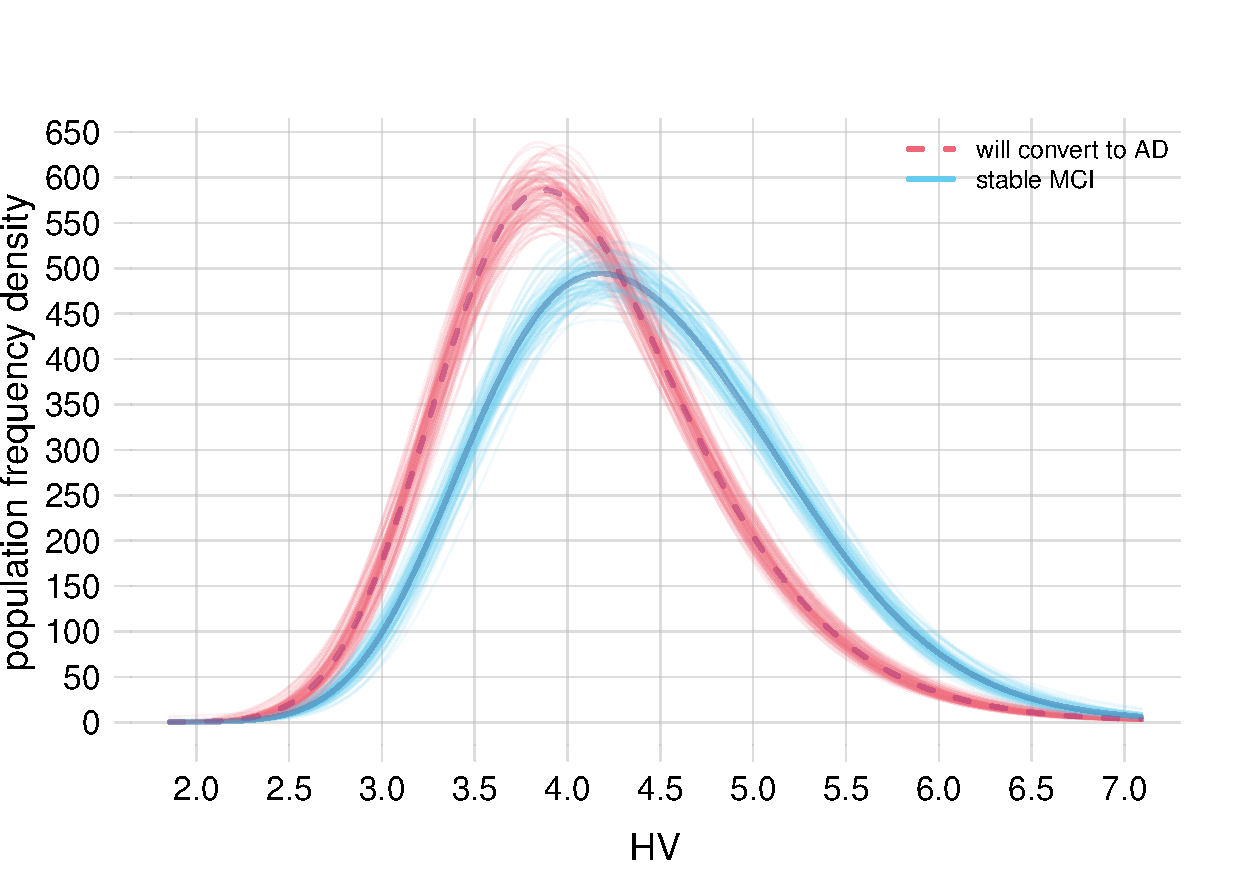
\includegraphics[width=0.45\linewidth]{figures/population_distr_HV.pdf}\hfill%
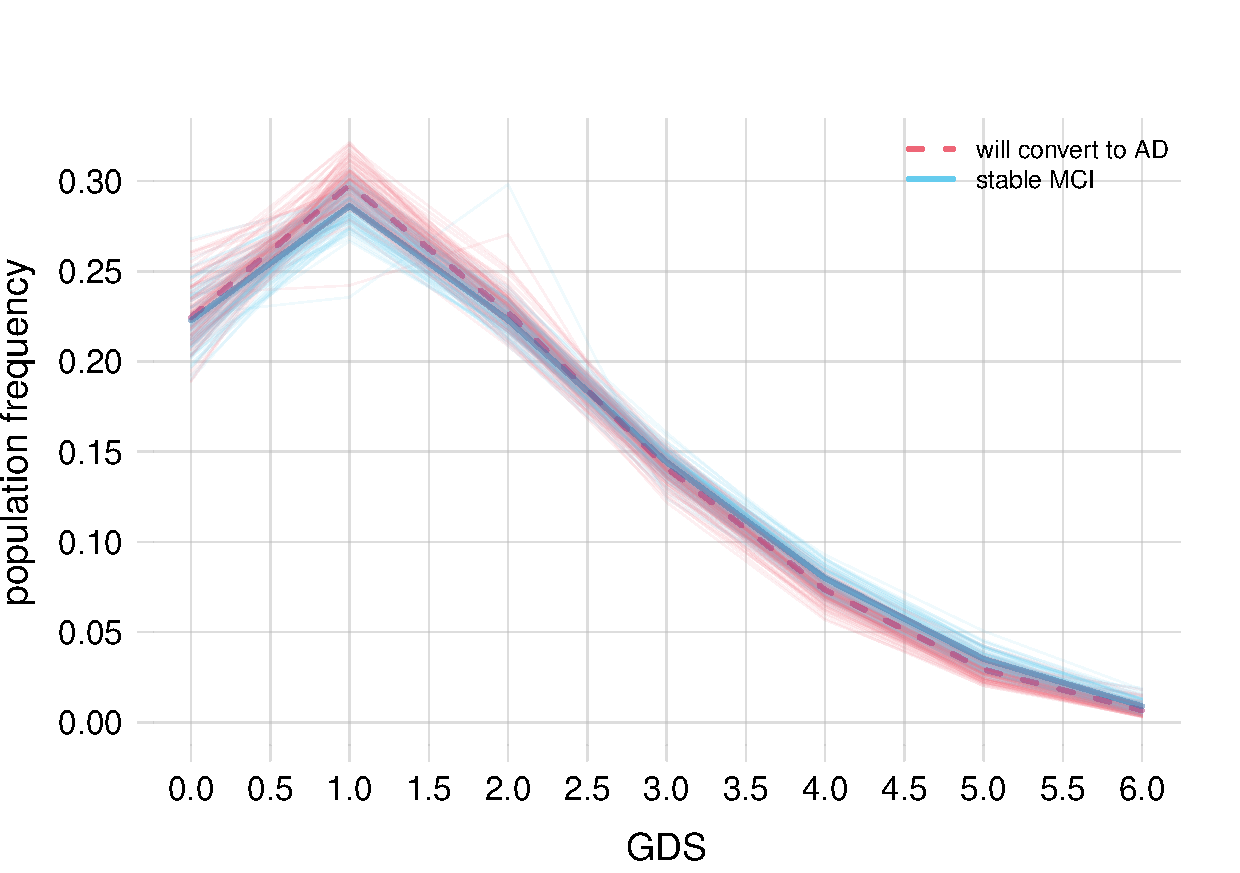
\includegraphics[width=0.45\linewidth]{figures/population_distr_GDS.pdf}%
\\ \caption{}\label{fig:distr}
\end{figure}
The package allows the user to visualize the probabilities above when just one predictand and one predictor variates are involved. If the results of the \texttt{Pr()} function are saved in some object, say \texttt{probs}, then the visualization is done by simply calling \texttt{plot(probs)}.

Figure~\ref{fig:distr} shows two examples from a study \citep{portamanaetal2023b} about conversion from Mild Cognitive Impairment (MCI) to Alzheimer's Disease (AD); they can be used to further illustrate the probability distributions~\eqref{eq:prob_var} and~\eqref{eq:prob_freq}.

In the plot on the left, the predictand variate is Hippocampal Volume ($\HV$); the predictor is the yes/no variate `will convert to AD' ($\cAD$). The thick solid blue line and thick dashed red line are the conditional probability distributions (omitting the sample-data dependence)
\begin{equation*}
  \P( \HV \| \cAD \mo \yn)\ ,\qquad
  \P( \HV \| \cAD \mo \yy) \ .
\end{equation*}
The cloud of thinner blue lines surrounding the first distribution above  represents the probability distribution
\begin{equation*}
  \P\bigl[ \yF(\HV \| \cAD \mo \yn)\bigr]
\end{equation*}
of possible frequency distributions; each thin line is a sample from this distribution.

Looking at this plot, a clinician can immediately see that the frequency distributions of hippocampal volume in the sub-populations of patients that will convert to Alzheimer's, and in those who will not, are different. Such a difference is almost certain even accounting for the uncertainty from the finite sample size. The plot on the right is analogous but for the predictand variate `Geriatric Depression Scale' ($\GDS$) in stead of hippocampal volume. In this case the clinician sees that the frequency distributions for the two sub-populations cannot be distinguished within the finite-sample uncertainty.

It is exactly this kind of differences and uncertainties that clinical researchers often try to clumsily capture through $p$-values. In private communications, several clinical researchers expressed elation at the capacity to visualize the estimates of different sub-population statistics, and even more the uncertainties they carry because of finite sample size.

The quick analysis above is mostly qualitative, but concrete numbers, such as quantiles and credibility intervals, expected values, and so on, can be easily produced. This becomes necessary when many variates are considered jointly and visualization is impossible. In such high-dimensional cases the package allows the user to compute the credibility intervals for any kind of distance between two frequency distributions (e.g. Hellinger or Kantorovich or Shannon-Jansen distance, or relative entropy). The computation of the mutual information between any two sets of variates, illustrated in a vignette\footnote{\url{https://pglpm.github.io/inferno/articles/mutualinfo.html}}, gives moreover a measure of their association that does not depend on assumptions such as linearity or gaussianity.

\begin{figure}[t]
\centering%
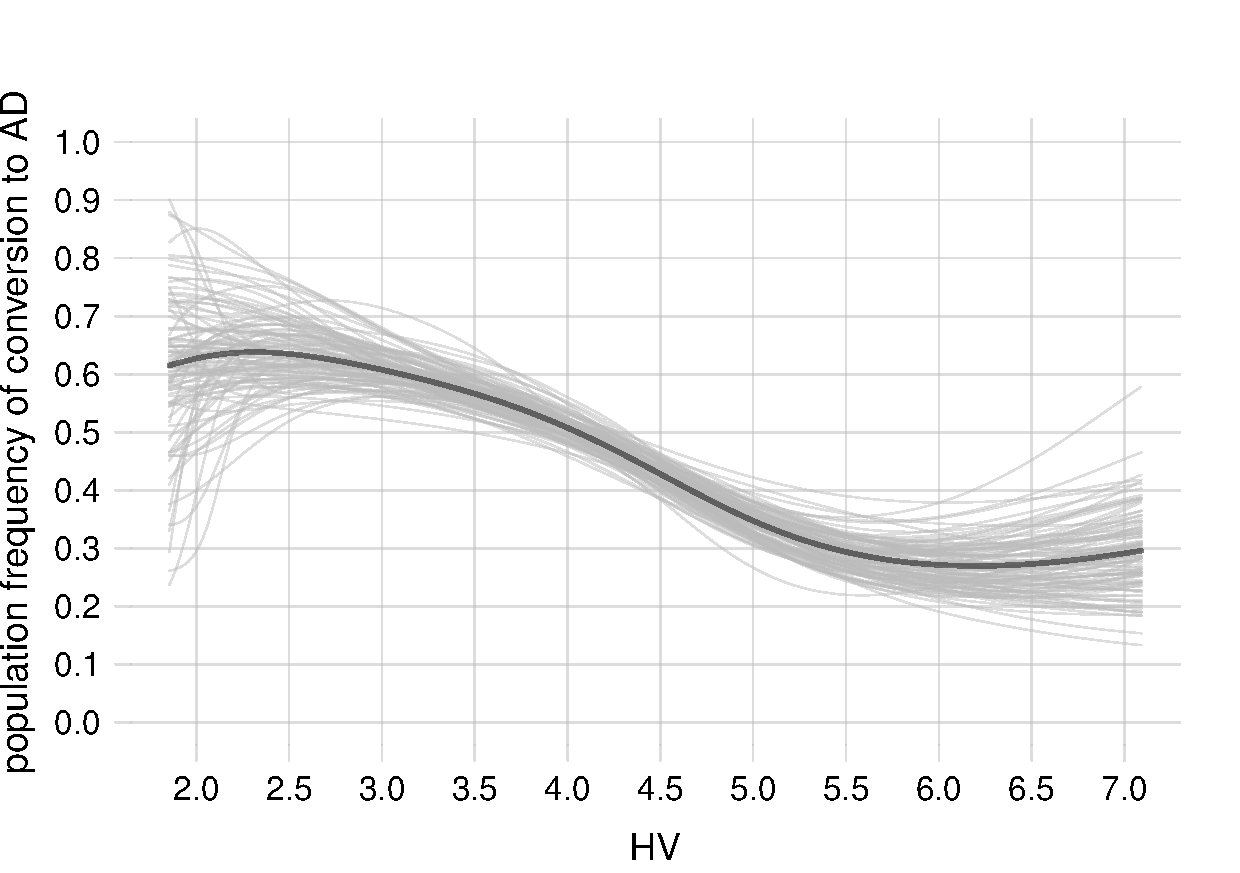
\includegraphics[width=0.45\linewidth]{figures/prob_conversion_HV.pdf}\hfill%
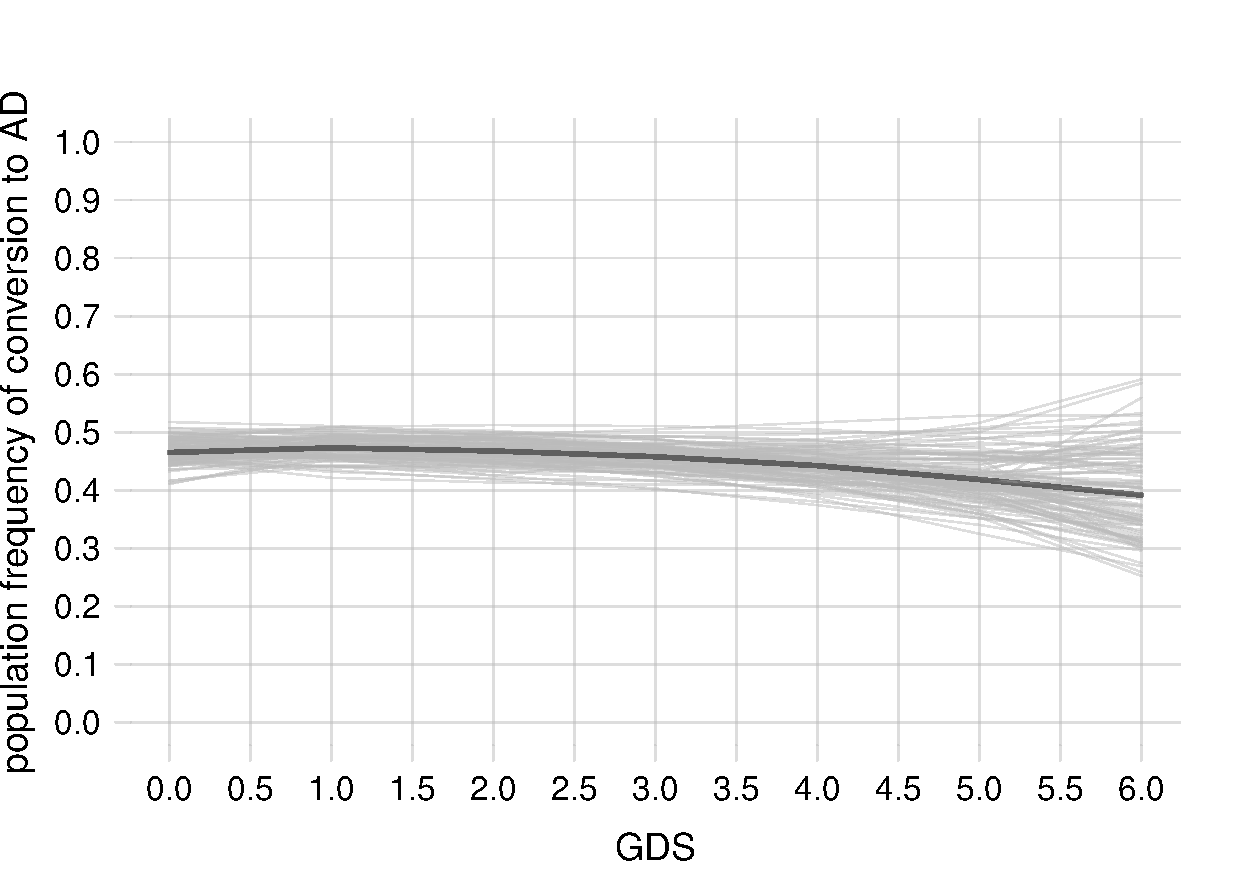
\includegraphics[width=0.45\linewidth]{figures/prob_conversion_GDS.pdf}%
\\ \caption{}\label{fig:distr_inv}
\end{figure}
The ability to swap the ``predictor'' and ``predictand'' roles of any variates is illustrated in the plots of fig.~\ref{fig:distr_inv}, parallel to those of fig.~\ref{fig:distr}. In the left plot, the thicker lines show the probabilities
\begin{equation*}
  \P( \cAD \mo \yy \| \HV)\
%  ,\qquad  \P( \cAD \mo \yy \| \GDS)
\end{equation*}
for various values of the $\HV$ variate, which is now a predictor.
% The clouds of thinner lines are samples of the corresponding probability distributions of the frequency distributions.
We see for example that among individuals having hippocampal volume around $5.0$, between 30\% and 40\% will convert to Alzheimer's. Among those with volume around $2.0$, we can only say that between roughly 45\% and 80\% will convert; in this case the finite-sample size (few samples with this $\HV$ value) leads to a much larger uncertainty of the frequency estimates.

The possibility of swapping predictor and predictand roles makes it also possible to implement, on the fly, corrections for base rates by means of Bayes's theorem \cite[\S\,4]{lindleyetal1981}.%\citep[\S\,3.2]{portamanaetal2023b}.

\medskip

Plots and calculations like the ones above are of course nothing new in Bayesian nonparametrics. The point here is that the user can produce them just by inputting the population sample in the package, waiting for the MCMC computation to finish, and then simply asking about variates of interest and plotting the results. The sequence of commands could be as simple as
\begin{verbatim}
learnt <- learn(data = 'data.csv', metadata = 'metadata.csv')
## Information about MCMC and expected end time...

probs <- Pr(Y = list(A = seq(0, 8, 0.1)), X = list(C = c('yes', 'no')), learnt)

plot(probs)
\end{verbatim}
More extensive use examples are given in the package's main vignette\footnote{\url{https://pglpm.github.io/inferno/articles/inferno_start.html}}. The package has also been used to ``calibrate'' the output of machine-learning algorithms \citep{dyrlandetal2022b}, improving their performance. Readers of the ISBA Bulletin are probably interested in the internals of the package, discussed next.


\subsection*{Internals}
\label{sec:representation}

In nonparametric population inference the prior and posterior probability distributions are over an in-principle infinite-dimensional manifold of frequency distributions. The mathematical representation of this manifold is therefore crucial. The \textbf{inferno} package uses the ingenious representation of a distribution as a mixture of product kernels discussed by Dunson \& Bhattacharya \citeyear{dunsonetal2011}. For example, a generic frequency distribution for variates $A$ and $B$ is written as
\begin{equation}
  \label{eq:mixture_kernel}
  \yF(A, B) = \sum_{i} w_{i}\, K_{A}(A \| \alpha_{i})\, K_{B}(B \| \beta_{i})
\end{equation}
where $w_{i}$ are normalized weights, $K_{A}$ a distribution for variate $A$ depending on parameters $\alpha_{i}$, and similarly for $K_{B}$. The product is easily generalized to any number of variates. In principle the sum should be countably infinite, but as discussed in Ishwaran \& Zarepour \citeyear{ishwaranetal2002c} it is possible to truncate it if an appropriate Dirichlet distribution is used for the weights $w_{i}$. Thus a frequency distribution $\yF$ is effectively represented, non-uniquely, by a very large but finite set of parameters $(w_{i}, \alpha_{i}, \beta_{i})$.

The representation above was somewhat deprecated in recent works which, however, consider inference problems where variates have clear predictor or predictand roles \citep[e.g.][]{wadeetal2014,wadeetal2014b}. As previously discussed, in many research fields there are no such a-priori roles; any variate could assume both. A representation that can easily swap the two roles  without overemphasizing either is therefore most appropriate. The representation~\eqref{eq:mixture_kernel} leads to very simple, symmetric, analytical expressions for the conditional of $A$ given $B$ and vice versa, and for any marginal:
\begin{equation*}
  \begin{gathered}
    \yF(A \| B) = \sum_{i}
    \frac{w_{i}\, K_{A}(A \| \alpha_{i})\, K_{B}(B \| \beta_{i})}{\sum_{j} w_{j}K_{B}(B \| \beta_{j})}
\qquad\qquad    \yF(B \| A) = \sum_{i}
    \frac{w_{i}\, K_{B}(B \| \beta_{i})\, K_{A}(A \| \alpha_{i})}{\sum_{j} w_{j}K_{A}(A \| \alpha_{j})}
    \\
    \yF(A) = \sum_{i}
    w_{i}\, K_{A}(A \| \alpha_{i}) \ .
  \end{gathered}
\end{equation*}
The (hyper)prior over the parameters representing the frequency distribution is a Dirichlet-process mixture. It allows for distributions having multiple, possibly sharp, peaks. For information about the kernels $K$ for different kinds of variates, and about the prior distribution, see the technical manual\footnote{\url{https://github.com/pglpm/inferno/raw/main/development/manual/optimal_predictor_machine.pdf}}.

\smallskip

The MCMC computation is based on Gibbs sampling; several chains are run in parallel. The stopping rule implements variations of the methods discussed in \cite{vehtarietal2021}. Regarding MCMC sampling, the package takes the following stance:

\textbullet\ For this kind of inference problems there is no need for tens of thousands or more independent MCMC samples (effective sample size). The package's default is just 3600. The mean of such samples is the probability~\eqref{eq:prob_var}, and the numerical uncertainty in this mean is thus around $\sqrt{3600} = 60$ times smaller than the ``variability'' of this probability, given by eq.~\eqref{eq:prob_freq}.

\textbullet\ It is acceptable that the sampling has not \emph{fully} converged (emphasis on `fully'). Why? Consider that machine-learning algorithms such as neural networks are effectively Bayesian nonparametric functional regressors, and their training is essentially an \emph{unconverged} Monte Carlo sampling \citep[see e.g.][]{mackay1992b,gal2016,mandtetal2017,huszar2017}. This ``sampling'' stops at a \emph{local} maximum of the posterior, and all samples are discarded. Thanks to this lack of convergence, neural-network training is fast; despite this lack of convergence, inferences can still be impressive. It is this writer's opinion that the same stance can and should at times be adopted in Bayesian nonparametrics: inferences can still be impressive and informative despite lack of full MCMC convergence, and superior to those of many machine-learning algorithms designed for the same task, as we found by using this package. And the uncertainty in the results can moreover be approximately assessed, instead of fully discarded as in neural-network training. So far, in applying \textbf{inferno} to concrete problems, we noticed that the MCMC sampling had converged in the majority of cases. In those in which it had not fully converged, the results were still correct to a good approximation, for example with credibility intervals that erred by less than 2\% from the converged values. This kind of approximate nonparametric results are still vastly superior to precise but opaque $p$-values.

These stances are motivated by the need for user-friendliness. The ultimate goal of the package is to let frequentist practitioners try and appreciate Bayesian methods (the package's main vignette is specially written for them); to let Bayesian-parametric practitioners try nonparametrics; and to show that Bayesian methods can be almost as fast and more powerful than many machine-learning approaches. Once the merits are seen, practitioners can slowly move to more complex Bayesian packages that allow for more control and custom problem-solving.

\textbf{inferno} has been already used and tested in several studies, but we'd like more testing before submitting it to CRAN. Testers and feedback are very welcome!

%\cite{selfetal1987}

%{\small%!TEX TS-program = pdflatex
\documentclass{article}
\usepackage[round]{natbib}
\usepackage{graphicx}
\usepackage{pifont,fancybox,multicol,palatcm}
\usepackage{caption}
\usepackage{float}
\usepackage{fancyhdr}
\usepackage{geometry}
\pagestyle{fancy} 
\geometry{margin=1.2in,top=1in,bottom=1in}
\usepackage{amsmath,amssymb}
\usepackage{bm}
\usepackage{textcomp}
\usepackage[usenames,dvipsnames]{color}
\usepackage[pdfmenubar=false,pdftex,pdfpagelabels=true,colorlinks=true,linkcolor=ISBABlue,citecolor=ISBABlue,urlcolor=DarkOrange]{hyperref}
\usepackage[export]{adjustbox}
\usepackage{soul}
\usepackage{wrapfig}
\usepackage{subcaption}
\usepackage{tabularx, booktabs}
%%%% Features this issue
\usepackage{pgfplots}
\usepackage{tikz}
\usepackage{url}
\usepackage{placeins}
%%%%




\graphicspath{{figures/}}

\usepackage{framed}
\makeatletter
\newenvironment{kframe}{%
 \def\at@end@of@kframe{}%
 \ifinner\ifhmode%
  \def\at@end@of@kframe{\end{minipage}}%
  \begin{minipage}{\columnwidth}%
 \fi\fi%
 \def\FrameCommand##1{\hskip\@totalleftmargin \hskip-\fboxsep
 \colorbox{shadecolor}{##1}\hskip-\fboxsep
     % There is no \\@totalrightmargin, so:
     \hskip-\linewidth \hskip-\@totalleftmargin \hskip\columnwidth}%
 \MakeFramed {\advance\hsize-\width
   \@totalleftmargin\z@ \linewidth\hsize
   \@setminipage}}%
 {\par\unskip\endMakeFramed%
 \at@end@of@kframe}
\makeatother

\parskip 1.5ex
\parindent 0em

\newcommand{\para}[1]{\vspace{.3em}\textbf{#1}\par}

\newcommand{\issue}{ISBA Bulletin, \textbf{32}(3), September 2025}
\newcommand{\blue}[1]{\textcolor{blue}{#1}}

\newcommand{\MyFilledBox}[1]{
\label{#1}
\vspace{1em}
\markright{\emph{#1}}{}
\hypertarget{#1}{}
\fcolorbox{White}{LightBlue}
{\begin{minipage}[t]{15.3cm}
\begin{center}

	\vspace{2.4mm}
	\subsection*{#1}

	\vspace{.3mm}
\end{center}
\end{minipage}}
\vspace{1mm}}

\newcommand{\MyFilledbox}[2]{
\hspace{-2.3mm}
\fcolorbox{White}{LightBlue}
{
\begin{minipage}[t]{#2}
	\begin{center}
	
		\textbf{\large #1}
	
	\end{center}
\end{minipage}}\\[2mm]}

\newcommand{\MyFancyBox}[3]{
\hspace{-4mm}
\fcolorbox{Black}{VeryLightBlue}{
\begin{minipage}[t]{#3}
	\MyFilledbox{#1}{#3}\\
	#2
\end{minipage}
}}

\newcommand{\MyFancyBoxWhite}[3]{
\hspace{-4mm}
\fcolorbox{Black}{White}{
\begin{minipage}[t]{#3}
	\MyFilledbox{#1}{#3}\\
	#2
\end{minipage}
}}

\renewcommand{\sectionmark}[1]{\markboth{#1}{}}

\definecolor{ISBABlue}{rgb}{0, .122, .388}
\definecolor{LightBlue}{rgb}{0.70, 0.75, 0.85}
\definecolor{VeryLightBlue}{rgb}{0.95,0.95,0.99}
\definecolor{DarkOrange}{rgb}{.9, 0.39, 0.0}

\fancyhead[L]{\issue}
\fancyhead[R]{}
\fancyfoot[C]{\thepage}
\fancyfoot[R]{\tt \href{https://www.bayesian.org}{www.bayesian.org}}

%---------- packages and commands for code blocks @software
\usepackage{mathtools}
\usepackage{fancyvrb}
\newcommand{\VerbBar}{|}
\newcommand{\VERB}{\Verb[commandchars=\\\{\}]}
\DefineVerbatimEnvironment{Highlighting}{Verbatim}{commandchars=\\\{\}}
% Add ',fontsize=\small' for more characters per line
\definecolor{shadecolor}{RGB}{248,248,248}
\newenvironment{Shaded}{\begin{snugshade}}{\end{snugshade}}
\newcommand{\AlertTok}[1]{\textcolor[rgb]{0.94,0.16,0.16}{#1}}
\newcommand{\AnnotationTok}[1]{\textcolor[rgb]{0.56,0.35,0.01}{\textbf{\textit{#1}}}}
\newcommand{\AttributeTok}[1]{\textcolor[rgb]{0.13,0.29,0.53}{#1}}
\newcommand{\BaseNTok}[1]{\textcolor[rgb]{0.00,0.00,0.81}{#1}}
\newcommand{\BuiltInTok}[1]{#1}
\newcommand{\CharTok}[1]{\textcolor[rgb]{0.31,0.60,0.02}{#1}}
\newcommand{\CommentTok}[1]{\textcolor[rgb]{0.56,0.35,0.01}{\textit{#1}}}
\newcommand{\CommentVarTok}[1]{\textcolor[rgb]{0.56,0.35,0.01}{\textbf{\textit{#1}}}}
\newcommand{\ConstantTok}[1]{\textcolor[rgb]{0.56,0.35,0.01}{#1}}
\newcommand{\ControlFlowTok}[1]{\textcolor[rgb]{0.13,0.29,0.53}{\textbf{#1}}}
\newcommand{\DataTypeTok}[1]{\textcolor[rgb]{0.13,0.29,0.53}{#1}}
\newcommand{\DecValTok}[1]{\textcolor[rgb]{0.00,0.00,0.81}{#1}}
\newcommand{\DocumentationTok}[1]{\textcolor[rgb]{0.56,0.35,0.01}{\textbf{\textit{#1}}}}
\newcommand{\ErrorTok}[1]{\textcolor[rgb]{0.64,0.00,0.00}{\textbf{#1}}}
\newcommand{\ExtensionTok}[1]{#1}
\newcommand{\FloatTok}[1]{\textcolor[rgb]{0.00,0.00,0.81}{#1}}
\newcommand{\FunctionTok}[1]{\textcolor[rgb]{0.13,0.29,0.53}{\textbf{#1}}}
\newcommand{\ImportTok}[1]{#1}
\newcommand{\InformationTok}[1]{\textcolor[rgb]{0.56,0.35,0.01}{\textbf{\textit{#1}}}}
\newcommand{\KeywordTok}[1]{\textcolor[rgb]{0.13,0.29,0.53}{\textbf{#1}}}
\newcommand{\NormalTok}[1]{#1}
\newcommand{\OperatorTok}[1]{\textcolor[rgb]{0.81,0.36,0.00}{\textbf{#1}}}
\newcommand{\OtherTok}[1]{\textcolor[rgb]{0.56,0.35,0.01}{#1}}
\newcommand{\PreprocessorTok}[1]{\textcolor[rgb]{0.56,0.35,0.01}{\textit{#1}}}
\newcommand{\RegionMarkerTok}[1]{#1}
\newcommand{\SpecialCharTok}[1]{\textcolor[rgb]{0.81,0.36,0.00}{\textbf{#1}}}
\newcommand{\SpecialStringTok}[1]{\textcolor[rgb]{0.31,0.60,0.02}{#1}}
\newcommand{\StringTok}[1]{\textcolor[rgb]{0.31,0.60,0.02}{#1}}
\newcommand{\VariableTok}[1]{\textcolor[rgb]{0.00,0.00,0.00}{#1}}
\newcommand{\VerbatimStringTok}[1]{\textcolor[rgb]{0.31,0.60,0.02}{#1}}
\newcommand{\WarningTok}[1]{\textcolor[rgb]{0.56,0.35,0.01}{\textbf{\textit{#1}}}}
%----------

\begin{document}
\hypertarget{TOP}{}
\thispagestyle{empty}
{\hfill \sc September 2025}

\vspace*{-.7em}
{\hfill \sc Vol.\ 32 No.\ 3}

\vspace*{-1.5em}
\begin{center}

\includegraphics[width=7cm]{isbalogo}
\end{center}
\fcolorbox{Black}{LightBlue}
{
\begin{minipage}[t]{15.1cm}
	\begin{center}	  
		\vspace{.5em}
%		\includegraphics[width=5cm]{isbalogotrans}\\[2em]
		\textbf{\Huge{ \sc{The \hspace{.1mm} ISBA\hspace{3mm} Bulletin}}}\\[2mm]
%		 		 {\sc Vol.\ 28 No.\ 1 \hfill  March 2021}\\[1pc] 				 
		 		 {\sc {\large Official bulletin of the International Society for Bayesian Analysis}}
		 		 \vspace{.5em}
	\end{center}
\end{minipage}
}


\clearpage

\newcommand{\citebi}{\cite}
\newcommand{\citein}[1]{\textnormal{\cite{#1}}}
\newcommand*{\subtitleproc}[1]{}
\newcommand*{\chapb}{}
\providecommand{\doi}[1]{}
\renewcommand{\doi}[1]{\href{https://doi.org/#1}{doi:#1}}
\newcommand*{\osfdoi}[1]{Open Science Framework \doi{#1}}
\newcommand*{\arxivdoi}[1]{arXiv \doi{#1}}
\newcommand*{\amp}{\&}
%% Probability macros
\renewcommand*{\P}{\mathrm{P}}%probability
\renewcommand*{\|}[1][]{\nonscript\:#1\vert\nonscript\:\mathopen{}}
\newcommand*{\mo}[1][=]{\mathclose{}\mathord{\nonscript\mkern0.5mu#1\nonscript\mkern0.5mu}\mathopen{}}
\newcommand*{\yF}{F}
\newcommand*{\yf}{f}
\newcommand*{\di}{\mathop{}\!\mathrm{d}}
%%
\newcommand*{\HV}{\mathit{HV}}
\newcommand*{\GDS}{\mathit{GDS}}
\newcommand*{\cAD}{\mathit{cAD}}
\newcommand*{\yy}{\mathrm{Y}}
\newcommand*{\yn}{\mathrm{N}}


\MyFilledBox{SOFTWARE HIGHLIGHT}
\begin{center}
  {\large Luca\enspace Porta Mana} \\
  Western Norway University of Applied Sciences\\
{\tt \href{mailto:pgl@portamana.org}{pgl@portamana.org}}


\Large
\textsc{inferno: INFERence in R with Bayesian NOnparametrics}
\end{center}

\subsection*{Population inference and Bayesian nonparametrics}
\label{sec:popinference}

A very important kind of inference in research fields such as medicine is \emph{population inference}, also called ``density inference'' or ``density regression''. Its general goal is to infer the frequency distribution of some variates in a population. This is different, for instance, from \emph{functional regression}, where the goal is to infer the functional relationship -- assumed to exist -- between a set of predictor variates and a target or ``predictand'' variate. In population inference the existence of a functional relation cannot be assumed. In fact there may not even be a clear distinction between predictor and predictand variates. A typical goal is the inference of frequency distributions within particular sub-populations or sub-groups; thus all sorts of conditional probabilities are required. A clinician may be interested in the statistics and probability of a medical condition given a symptom, but also in that of a symptom given a medical condition; and maybe only within subjects of a given sex or age. De~Finetti's theorem \citep[see e.g.][\S\S\,4.2, 4.3, 4.6]{bernardoetal1994_r2000} lies at the heart of population-inference methods; a particularly brilliant discussion is given by Lindley \& Novick \citeyearpar{lindleyetal1981}.

Sadly many researchers still approach population-inference problems by means of $p$-values or other frequentist practices, which only give limited, coarse, and not seldom misleading results about a population's frequency distribution. Some researchers adopt Bayesian methods but limit themselves to \emph{parametric} ones, which make very restrictive and possibly unrealistic assumptions about the population's distribution; as opposed to \emph{nonparametric} ones, which do not.

Until a couple decades ago the use of parametric methods, and maybe even of frequentist practices, had pragmatic reasons. Better methods were computationally too costly or unfeasible. Population-inference problems were low-dimensional; one could \emph{visually} check whether the assumptions were appropriate and the results reasonable. But today these reasons cannot earnestly be given \citep{walker2010}. Bayesian nonparametric methods have become computationally feasible for many kinds of inference. Many inference problems today involve from tens to thousands of variates; it is impossible to visually check in such high-dimensional spaces whether frequentist practices or parametric assumptions are acceptable, or by how much they err. Results may be affected by large parametric-modelling errors \citep{draper1995}.

But there is still one reason today for why Bayesian nonparametric methods are avoided: \emph{lack of user-friendly software}. Many clinical researchers might like to try a Bayesian nonparametric analysis, but cannot: they would need to study Markov-chain Monte Carlo (MCMC) techniques, programming languages to implement the latter, and a read about plethora of debated practices to ``assess convergence''. Most clinicians do not have time to learn all this even if they wanted to. Also, available packages for Bayesian nonparametrics are not quite suited to population inference. Some of them focus on functional regression, which as discussed above is not an appropriate assumption. Some make a priori distinctions between predictor and predictand variates, limiting the range of useful inferences. Most still require MCMC programming expertise.

The R-package \textbf{inferno}\footnote{\url{https://pglpm.github.io/inferno/}} was built to try to remedy the lack of user-friendly software of this kind.

\subsection*{Use and features}
\label{sec:features}

Using the package is simple. The user first provides a data sample $S$ of variates from a population, for instance age, sex, symptom, disease, and kind of treatment of a number of patients that satisfy specific criteria. The package can work with any combination of continuous, discrete ordinal, nominal, and binary variates. Continuous variates can be defined in bounded intervals, and can also have boundary values with finite probability mass, as it may happen with censoring. The package cannot handle periodic variates yet, or variates with complex topology, such as images. The data sample and the variate characteristics (type, domain, possible censoring) are provided by the user as two CSV files to an R function called \texttt{learn()}.

The package then runs a MCMC computation by means of the \textbf{Nimble} package\footnote{\url{https://r-nimble.org/}}, using parallel CPUs if available, to find the probability distribution over all possible joint frequency distributions of the variates. The result is saved in an R object called \texttt{learnt}. The crucial point here is that this computation is automatic and does not require any further control from the user, who is simply informed at regular intervals about the expected end time of the computation. (Optional arguments still allow users expert in MCMC to control many parameters such as number of chains, target effective sample size, thinning and burn-in, and even some hyperprior parameters.)

Once the computation has finished, the user can inquire multiple times about any of the following:
\vspace{-\topsep}
\setlength{\leftmargini}{17.62pt}
\begin{itemize}
  \itemsep0.5ex
\item For a new unit of the population, say a new patient, the conditional probability (density) for the values of \emph{any} set of variates $A \mo a, B \mo b, \dotso$ given \emph{any} other set $C \mo c, D \mo d, \dotso$:
  \begin{equation}\label{eq:prob_var}
    \P(A \mo a, B \mo b, \dotso \|C \mo c, D \mo d, \dotso , S)
  \end{equation}
  Such a probability could for instance be used in medical decision making \citep{soxetal1988_r2024,huninketal2001_r2014}. The conditional can be empty; tail probabilities (e.g.\ $A \ge a$, $C \le c$) can also be requested.

\item The probability distribution for the conditional \emph{frequencies}, in the whole unsampled population, of the values of any set of variates given any other set (possibly empty). If we denote the frequency distribution by $\yF$ and a specific value by $\yf$, this probability can be written
  \begin{equation}\label{eq:prob_freq}
    \P\bigl[ \yF(A \mo a, \dotso \|C \mo c, \dotso) = \yf \|[\big] S\bigr]
    \,\di\yf \ .
  \end{equation}
This probability distribution is represented by the MCMC samples $\yf_{i}$ drawn from it by \texttt{learn()}.

\item The mutual information \citep[Ch.~8]{mackay1995_r2005} between any two sets of quantities.
\end{itemize}
\vspace{-\topsep}

Probabilities~\eqref{eq:prob_var} and~\eqref{eq:prob_freq} are connected by a variant of de~Finetti's theorem:
\begin{equation}
  \label{eq:definetti1}
  \P(A \mo a, \dotso \|C \mo c, \dotso , S)  =
  \int \yf \,
  \P\bigl[ \yF(A \mo a, \dotso \|C \mo c, \dotso) = \yf \|[\big] S\bigr]
  \,\di\yf \ .
\end{equation}

In a manner of speaking, the probability distribution~\eqref{eq:prob_freq} expresses how much the probability value~\eqref{eq:prob_var} could change, if it were updated by sampling the whole population. It expresses the uncertainty in the statistical results owing to finite sample size.

The package function \texttt{Pr(Y, X, learnt)} does the first two kinds of calculations. The user provides a list \texttt{Y} of predictand variates and values of interest; an optional, analogous list \texttt{X} of predictors; and the \texttt{learnt} object produced by \texttt{learn()}. The calculation of mutual information is done by the package function \texttt{mutualinfo(Y1names, Y2names, X)}, where the first two arguments are the variate sets of interest, and the optional third argument is a set of variate values to conditionalize upon.

\medskip

\begin{figure}[t]
\centering%
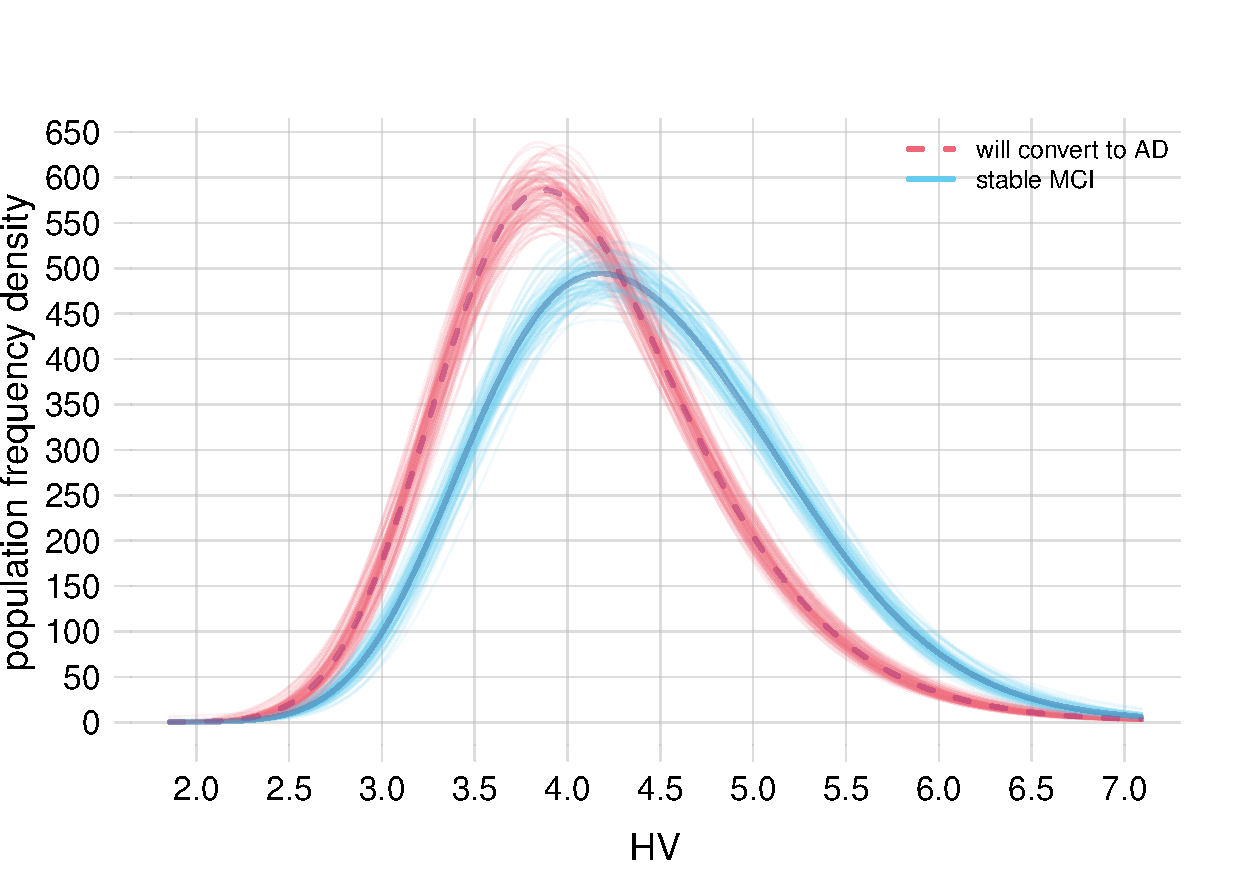
\includegraphics[width=0.45\linewidth]{figures/population_distr_HV.pdf}\hfill%
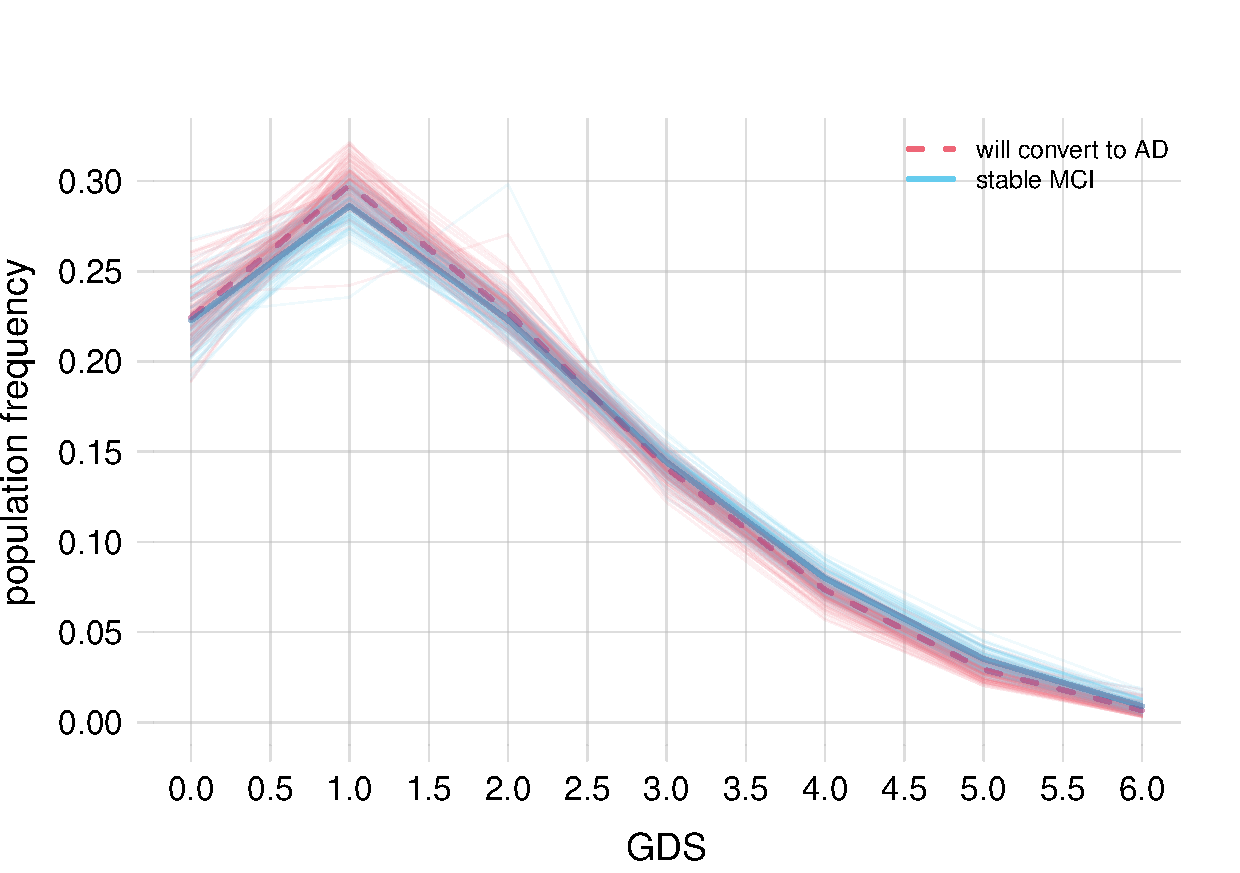
\includegraphics[width=0.45\linewidth]{figures/population_distr_GDS.pdf}%
\\ \caption{}\label{fig:distr}
\end{figure}
The package allows the user to visualize the probabilities above when just one predictand and one predictor variates are involved. If the results of the \texttt{Pr()} function are saved in some object, say \texttt{probs}, then the visualization is done by simply calling \texttt{plot(probs)}.

Figure~\ref{fig:distr} shows two examples from a study \citep{portamanaetal2023b} about conversion from Mild Cognitive Impairment (MCI) to Alzheimer's Disease (AD); they can be used to further illustrate the probability distributions~\eqref{eq:prob_var} and~\eqref{eq:prob_freq}.

In the plot on the left, the predictand variate is Hippocampal Volume ($\HV$); the predictor is the yes/no variate `will convert to AD' ($\cAD$). The thick solid blue line and thick dashed red line are the conditional probability distributions (omitting the sample-data dependence)
\begin{equation*}
  \P( \HV \| \cAD \mo \yn)\ ,\qquad
  \P( \HV \| \cAD \mo \yy) \ .
\end{equation*}
The cloud of thinner blue lines surrounding the first distribution above  represents the probability distribution
\begin{equation*}
  \P\bigl[ \yF(\HV \| \cAD \mo \yn)\bigr]
\end{equation*}
of possible frequency distributions; each thin line is a sample from this distribution.

Looking at this plot, a clinician can immediately see that the frequency distributions of hippocampal volume in the sub-populations of patients that will convert to Alzheimer's, and in those who will not, are different. Such a difference is almost certain even accounting for the uncertainty from the finite sample size. The plot on the right is analogous but for the predictand variate `Geriatric Depression Scale' ($\GDS$) in stead of hippocampal volume. In this case the clinician sees that the frequency distributions for the two sub-populations cannot be distinguished within the finite-sample uncertainty.

It is exactly this kind of differences and uncertainties that clinical researchers often try to clumsily capture through $p$-values. In private communications, several clinical researchers expressed elation at the capacity to visualize the estimates of different sub-population statistics, and even more the uncertainties they carry because of finite sample size.

The quick analysis above is mostly qualitative, but concrete numbers, such as quantiles and credibility intervals, expected values, and so on, can be easily produced. This becomes necessary when many variates are considered jointly and visualization is impossible. In such high-dimensional cases the package allows the user to compute the credibility intervals for any kind of distance between two frequency distributions (e.g. Hellinger or Kantorovich or Shannon-Jansen distance, or relative entropy). The computation of the mutual information between any two sets of variates, illustrated in a vignette\footnote{\url{https://pglpm.github.io/inferno/articles/mutualinfo.html}}, gives moreover a measure of their association that does not depend on assumptions such as linearity or gaussianity.

\begin{figure}[t]
\centering%
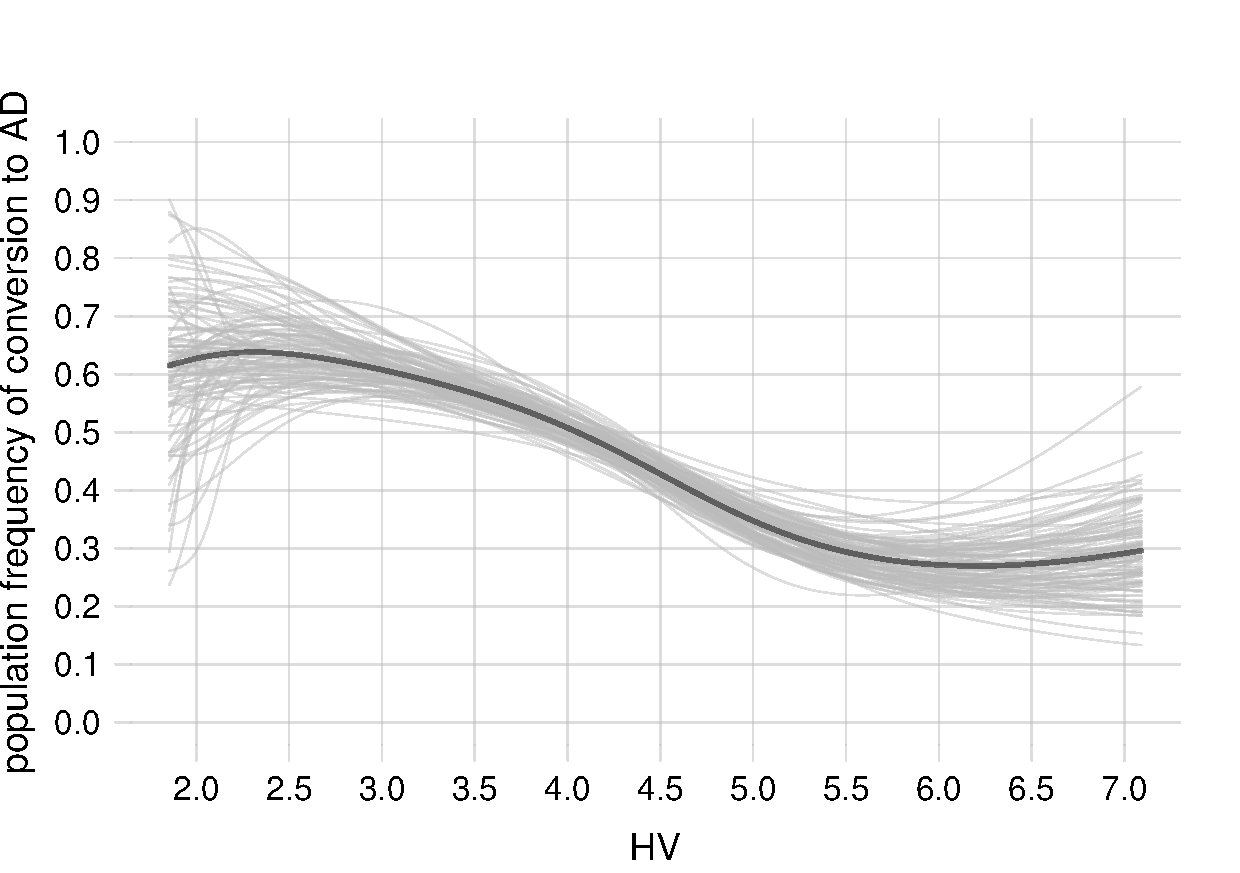
\includegraphics[width=0.45\linewidth]{figures/prob_conversion_HV.pdf}\hfill%
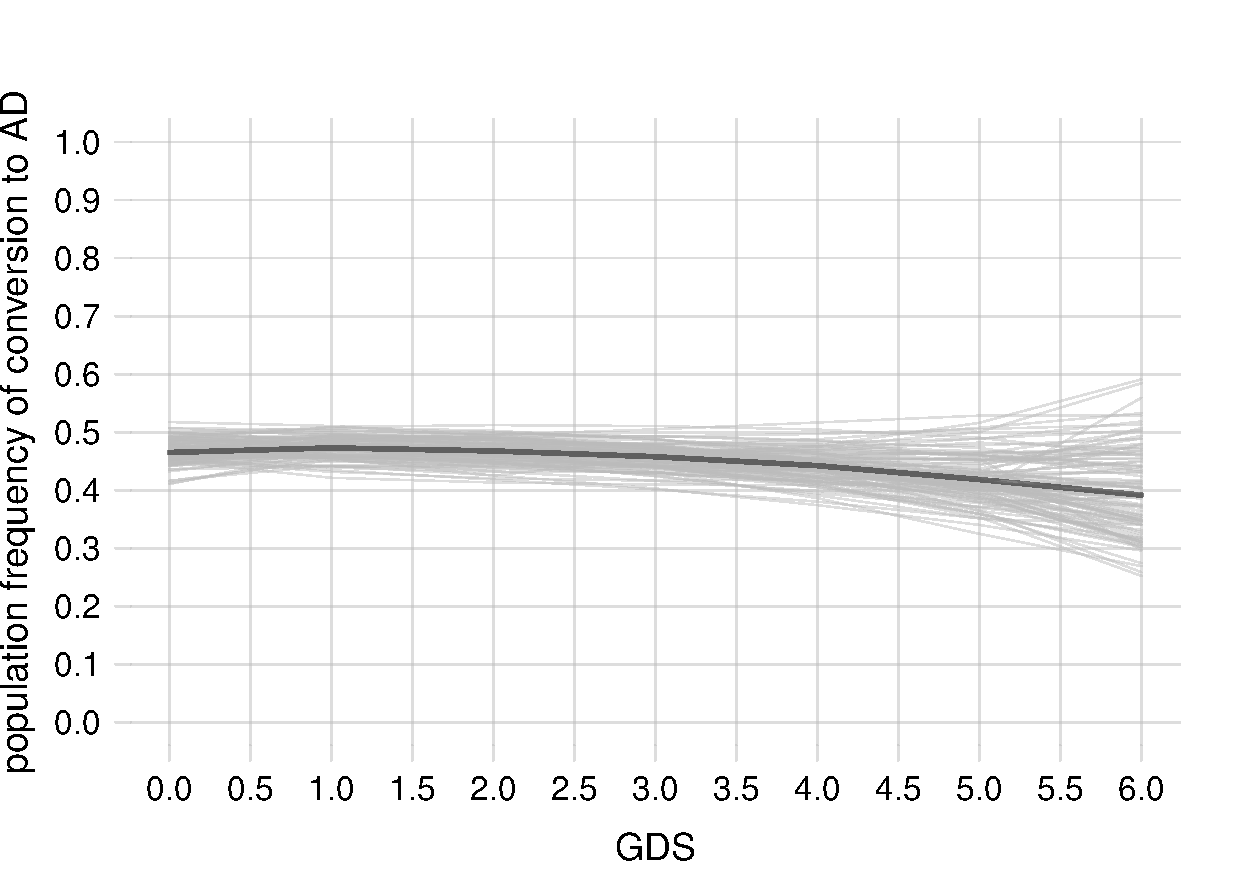
\includegraphics[width=0.45\linewidth]{figures/prob_conversion_GDS.pdf}%
\\ \caption{}\label{fig:distr_inv}
\end{figure}
The ability to swap the ``predictor'' and ``predictand'' roles of any variates is illustrated in the plots of fig.~\ref{fig:distr_inv}, parallel to those of fig.~\ref{fig:distr}. In the left plot, the thicker lines show the probabilities
\begin{equation*}
  \P( \cAD \mo \yy \| \HV)\
%  ,\qquad  \P( \cAD \mo \yy \| \GDS)
\end{equation*}
for various values of the $\HV$ variate, which is now a predictor.
% The clouds of thinner lines are samples of the corresponding probability distributions of the frequency distributions.
We see for example that among individuals having hippocampal volume around $5.0$, between 30\% and 40\% will convert to Alzheimer's. Among those with volume around $2.0$, we can only say that between roughly 45\% and 80\% will convert; in this case the finite-sample size (few samples with this $\HV$ value) leads to a much larger uncertainty of the frequency estimates.

The possibility of swapping predictor and predictand roles makes it also possible to implement, on the fly, corrections for base rates by means of Bayes's theorem \cite[\S\,4]{lindleyetal1981}.%\citep[\S\,3.2]{portamanaetal2023b}.

\medskip

Plots and calculations like the ones above are of course nothing new in Bayesian nonparametrics. The point here is that the user can produce them just by inputting the population sample in the package, waiting for the MCMC computation to finish, and then simply asking about variates of interest and plotting the results. The sequence of commands could be as simple as
\begin{verbatim}
learnt <- learn(data = 'data.csv', metadata = 'metadata.csv')
## Information about MCMC and expected end time...

probs <- Pr(Y = list(A = seq(0, 8, 0.1)), X = list(C = c('yes', 'no')), learnt)

plot(probs)
\end{verbatim}
More extensive use examples are given in the package's main vignette\footnote{\url{https://pglpm.github.io/inferno/articles/inferno_start.html}}. The package has also been used to ``calibrate'' the output of machine-learning algorithms \citep{dyrlandetal2022b}, improving their performance. Readers of the ISBA Bulletin are probably interested in the internals of the package, discussed next.


\subsection*{Internals}
\label{sec:representation}

In nonparametric population inference the prior and posterior probability distributions are over an in-principle infinite-dimensional manifold of frequency distributions. The mathematical representation of this manifold is therefore crucial. The \textbf{inferno} package uses the ingenious representation of a distribution as a mixture of product kernels discussed by Dunson \& Bhattacharya \citeyear{dunsonetal2011}. For example, a generic frequency distribution for variates $A$ and $B$ is written as
\begin{equation}
  \label{eq:mixture_kernel}
  \yF(A, B) = \sum_{i} w_{i}\, K_{A}(A \| \alpha_{i})\, K_{B}(B \| \beta_{i})
\end{equation}
where $w_{i}$ are normalized weights, $K_{A}$ a distribution for variate $A$ depending on parameters $\alpha_{i}$, and similarly for $K_{B}$. The product is easily generalized to any number of variates. In principle the sum should be countably infinite, but as discussed in Ishwaran \& Zarepour \citeyear{ishwaranetal2002c} it is possible to truncate it if an appropriate Dirichlet distribution is used for the weights $w_{i}$. Thus a frequency distribution $\yF$ is effectively represented, non-uniquely, by a very large but finite set of parameters $(w_{i}, \alpha_{i}, \beta_{i})$.

The representation above was somewhat deprecated in recent works which, however, consider inference problems where variates have clear predictor or predictand roles \citep[e.g.][]{wadeetal2014,wadeetal2014b}. As previously discussed, in many research fields there are no such a-priori roles; any variate could assume both. A representation that can easily swap the two roles  without overemphasizing either is therefore most appropriate. The representation~\eqref{eq:mixture_kernel} leads to very simple, symmetric, analytical expressions for the conditional of $A$ given $B$ and vice versa, and for any marginal:
\begin{equation*}
  \begin{gathered}
    \yF(A \| B) = \sum_{i}
    \frac{w_{i}\, K_{A}(A \| \alpha_{i})\, K_{B}(B \| \beta_{i})}{\sum_{j} w_{j}K_{B}(B \| \beta_{j})}
\qquad\qquad    \yF(B \| A) = \sum_{i}
    \frac{w_{i}\, K_{B}(B \| \beta_{i})\, K_{A}(A \| \alpha_{i})}{\sum_{j} w_{j}K_{A}(A \| \alpha_{j})}
    \\
    \yF(A) = \sum_{i}
    w_{i}\, K_{A}(A \| \alpha_{i}) \ .
  \end{gathered}
\end{equation*}
The (hyper)prior over the parameters representing the frequency distribution is a Dirichlet-process mixture. It allows for distributions having multiple, possibly sharp, peaks. For information about the kernels $K$ for different kinds of variates, and about the prior distribution, see the technical manual\footnote{\url{https://github.com/pglpm/inferno/raw/main/development/manual/optimal_predictor_machine.pdf}}.

\smallskip

The MCMC computation is based on Gibbs sampling; several chains are run in parallel. The stopping rule implements variations of the methods discussed in \cite{vehtarietal2021}. Regarding MCMC sampling, the package takes the following stance:

\textbullet\ For this kind of inference problems there is no need for tens of thousands or more independent MCMC samples (effective sample size). The package's default is just 3600. The mean of such samples is the probability~\eqref{eq:prob_var}, and the numerical uncertainty in this mean is thus around $\sqrt{3600} = 60$ times smaller than the ``variability'' of this probability, given by eq.~\eqref{eq:prob_freq}.

\textbullet\ It is acceptable that the sampling has not \emph{fully} converged (emphasis on `fully'). Why? Consider that machine-learning algorithms such as neural networks are effectively Bayesian nonparametric functional regressors, and their training is essentially an \emph{unconverged} Monte Carlo sampling \citep[see e.g.][]{mackay1992b,gal2016,mandtetal2017,huszar2017}. This ``sampling'' stops at a \emph{local} maximum of the posterior, and all samples are discarded. Thanks to this lack of convergence, neural-network training is fast; despite this lack of convergence, inferences can still be impressive. It is this writer's opinion that the same stance can and should at times be adopted in Bayesian nonparametrics: inferences can still be impressive and informative despite lack of full MCMC convergence, and superior to those of many machine-learning algorithms designed for the same task, as we found by using this package. And the uncertainty in the results can moreover be approximately assessed, instead of fully discarded as in neural-network training. So far, in applying \textbf{inferno} to concrete problems, we noticed that the MCMC sampling had converged in the majority of cases. In those in which it had not fully converged, the results were still correct to a good approximation, for example with credibility intervals that erred by less than 2\% from the converged values. This kind of approximate nonparametric results are still vastly superior to precise but opaque $p$-values.

These stances are motivated by the need for user-friendliness. The ultimate goal of the package is to let frequentist practitioners try and appreciate Bayesian methods (the package's main vignette is specially written for them); to let Bayesian-parametric practitioners try nonparametrics; and to show that Bayesian methods can be almost as fast and more powerful than many machine-learning approaches. Once the merits are seen, practitioners can slowly move to more complex Bayesian packages that allow for more control and custom problem-solving.

\textbf{inferno} has been already used and tested in several studies, but we'd like more testing before submitting it to CRAN. Testers and feedback are very welcome!


%{\small%!TEX TS-program = pdflatex
\documentclass{article}
\usepackage[round]{natbib}
\usepackage{graphicx}
\usepackage{pifont,fancybox,multicol,palatcm}
\usepackage{caption}
\usepackage{float}
\usepackage{fancyhdr}
\usepackage{geometry}
\pagestyle{fancy} 
\geometry{margin=1.2in,top=1in,bottom=1in}
\usepackage{amsmath,amssymb}
\usepackage{bm}
\usepackage{textcomp}
\usepackage[usenames,dvipsnames]{color}
\usepackage[pdfmenubar=false,pdftex,pdfpagelabels=true,colorlinks=true,linkcolor=ISBABlue,citecolor=ISBABlue,urlcolor=DarkOrange]{hyperref}
\usepackage[export]{adjustbox}
\usepackage{soul}
\usepackage{wrapfig}
\usepackage{subcaption}
\usepackage{tabularx, booktabs}
%%%% Features this issue
\usepackage{pgfplots}
\usepackage{tikz}
\usepackage{url}
\usepackage{placeins}
%%%%




\graphicspath{{figures/}}

\usepackage{framed}
\makeatletter
\newenvironment{kframe}{%
 \def\at@end@of@kframe{}%
 \ifinner\ifhmode%
  \def\at@end@of@kframe{\end{minipage}}%
  \begin{minipage}{\columnwidth}%
 \fi\fi%
 \def\FrameCommand##1{\hskip\@totalleftmargin \hskip-\fboxsep
 \colorbox{shadecolor}{##1}\hskip-\fboxsep
     % There is no \\@totalrightmargin, so:
     \hskip-\linewidth \hskip-\@totalleftmargin \hskip\columnwidth}%
 \MakeFramed {\advance\hsize-\width
   \@totalleftmargin\z@ \linewidth\hsize
   \@setminipage}}%
 {\par\unskip\endMakeFramed%
 \at@end@of@kframe}
\makeatother

\parskip 1.5ex
\parindent 0em

\newcommand{\para}[1]{\vspace{.3em}\textbf{#1}\par}

\newcommand{\issue}{ISBA Bulletin, \textbf{32}(3), September 2025}
\newcommand{\blue}[1]{\textcolor{blue}{#1}}

\newcommand{\MyFilledBox}[1]{
\label{#1}
\vspace{1em}
\markright{\emph{#1}}{}
\hypertarget{#1}{}
\fcolorbox{White}{LightBlue}
{\begin{minipage}[t]{15.3cm}
\begin{center}

	\vspace{2.4mm}
	\subsection*{#1}

	\vspace{.3mm}
\end{center}
\end{minipage}}
\vspace{1mm}}

\newcommand{\MyFilledbox}[2]{
\hspace{-2.3mm}
\fcolorbox{White}{LightBlue}
{
\begin{minipage}[t]{#2}
	\begin{center}
	
		\textbf{\large #1}
	
	\end{center}
\end{minipage}}\\[2mm]}

\newcommand{\MyFancyBox}[3]{
\hspace{-4mm}
\fcolorbox{Black}{VeryLightBlue}{
\begin{minipage}[t]{#3}
	\MyFilledbox{#1}{#3}\\
	#2
\end{minipage}
}}

\newcommand{\MyFancyBoxWhite}[3]{
\hspace{-4mm}
\fcolorbox{Black}{White}{
\begin{minipage}[t]{#3}
	\MyFilledbox{#1}{#3}\\
	#2
\end{minipage}
}}

\renewcommand{\sectionmark}[1]{\markboth{#1}{}}

\definecolor{ISBABlue}{rgb}{0, .122, .388}
\definecolor{LightBlue}{rgb}{0.70, 0.75, 0.85}
\definecolor{VeryLightBlue}{rgb}{0.95,0.95,0.99}
\definecolor{DarkOrange}{rgb}{.9, 0.39, 0.0}

\fancyhead[L]{\issue}
\fancyhead[R]{}
\fancyfoot[C]{\thepage}
\fancyfoot[R]{\tt \href{https://www.bayesian.org}{www.bayesian.org}}

%---------- packages and commands for code blocks @software
\usepackage{mathtools}
\usepackage{fancyvrb}
\newcommand{\VerbBar}{|}
\newcommand{\VERB}{\Verb[commandchars=\\\{\}]}
\DefineVerbatimEnvironment{Highlighting}{Verbatim}{commandchars=\\\{\}}
% Add ',fontsize=\small' for more characters per line
\definecolor{shadecolor}{RGB}{248,248,248}
\newenvironment{Shaded}{\begin{snugshade}}{\end{snugshade}}
\newcommand{\AlertTok}[1]{\textcolor[rgb]{0.94,0.16,0.16}{#1}}
\newcommand{\AnnotationTok}[1]{\textcolor[rgb]{0.56,0.35,0.01}{\textbf{\textit{#1}}}}
\newcommand{\AttributeTok}[1]{\textcolor[rgb]{0.13,0.29,0.53}{#1}}
\newcommand{\BaseNTok}[1]{\textcolor[rgb]{0.00,0.00,0.81}{#1}}
\newcommand{\BuiltInTok}[1]{#1}
\newcommand{\CharTok}[1]{\textcolor[rgb]{0.31,0.60,0.02}{#1}}
\newcommand{\CommentTok}[1]{\textcolor[rgb]{0.56,0.35,0.01}{\textit{#1}}}
\newcommand{\CommentVarTok}[1]{\textcolor[rgb]{0.56,0.35,0.01}{\textbf{\textit{#1}}}}
\newcommand{\ConstantTok}[1]{\textcolor[rgb]{0.56,0.35,0.01}{#1}}
\newcommand{\ControlFlowTok}[1]{\textcolor[rgb]{0.13,0.29,0.53}{\textbf{#1}}}
\newcommand{\DataTypeTok}[1]{\textcolor[rgb]{0.13,0.29,0.53}{#1}}
\newcommand{\DecValTok}[1]{\textcolor[rgb]{0.00,0.00,0.81}{#1}}
\newcommand{\DocumentationTok}[1]{\textcolor[rgb]{0.56,0.35,0.01}{\textbf{\textit{#1}}}}
\newcommand{\ErrorTok}[1]{\textcolor[rgb]{0.64,0.00,0.00}{\textbf{#1}}}
\newcommand{\ExtensionTok}[1]{#1}
\newcommand{\FloatTok}[1]{\textcolor[rgb]{0.00,0.00,0.81}{#1}}
\newcommand{\FunctionTok}[1]{\textcolor[rgb]{0.13,0.29,0.53}{\textbf{#1}}}
\newcommand{\ImportTok}[1]{#1}
\newcommand{\InformationTok}[1]{\textcolor[rgb]{0.56,0.35,0.01}{\textbf{\textit{#1}}}}
\newcommand{\KeywordTok}[1]{\textcolor[rgb]{0.13,0.29,0.53}{\textbf{#1}}}
\newcommand{\NormalTok}[1]{#1}
\newcommand{\OperatorTok}[1]{\textcolor[rgb]{0.81,0.36,0.00}{\textbf{#1}}}
\newcommand{\OtherTok}[1]{\textcolor[rgb]{0.56,0.35,0.01}{#1}}
\newcommand{\PreprocessorTok}[1]{\textcolor[rgb]{0.56,0.35,0.01}{\textit{#1}}}
\newcommand{\RegionMarkerTok}[1]{#1}
\newcommand{\SpecialCharTok}[1]{\textcolor[rgb]{0.81,0.36,0.00}{\textbf{#1}}}
\newcommand{\SpecialStringTok}[1]{\textcolor[rgb]{0.31,0.60,0.02}{#1}}
\newcommand{\StringTok}[1]{\textcolor[rgb]{0.31,0.60,0.02}{#1}}
\newcommand{\VariableTok}[1]{\textcolor[rgb]{0.00,0.00,0.00}{#1}}
\newcommand{\VerbatimStringTok}[1]{\textcolor[rgb]{0.31,0.60,0.02}{#1}}
\newcommand{\WarningTok}[1]{\textcolor[rgb]{0.56,0.35,0.01}{\textbf{\textit{#1}}}}
%----------

\begin{document}
\hypertarget{TOP}{}
\thispagestyle{empty}
{\hfill \sc September 2025}

\vspace*{-.7em}
{\hfill \sc Vol.\ 32 No.\ 3}

\vspace*{-1.5em}
\begin{center}

\includegraphics[width=7cm]{isbalogo}
\end{center}
\fcolorbox{Black}{LightBlue}
{
\begin{minipage}[t]{15.1cm}
	\begin{center}	  
		\vspace{.5em}
%		\includegraphics[width=5cm]{isbalogotrans}\\[2em]
		\textbf{\Huge{ \sc{The \hspace{.1mm} ISBA\hspace{3mm} Bulletin}}}\\[2mm]
%		 		 {\sc Vol.\ 28 No.\ 1 \hfill  March 2021}\\[1pc] 				 
		 		 {\sc {\large Official bulletin of the International Society for Bayesian Analysis}}
		 		 \vspace{.5em}
	\end{center}
\end{minipage}
}


\clearpage

\newcommand{\citebi}{\cite}
\newcommand{\citein}[1]{\textnormal{\cite{#1}}}
\newcommand*{\subtitleproc}[1]{}
\newcommand*{\chapb}{}
\providecommand{\doi}[1]{}
\renewcommand{\doi}[1]{\href{https://doi.org/#1}{doi:#1}}
\newcommand*{\osfdoi}[1]{Open Science Framework \doi{#1}}
\newcommand*{\arxivdoi}[1]{arXiv \doi{#1}}
\newcommand*{\amp}{\&}
%% Probability macros
\renewcommand*{\P}{\mathrm{P}}%probability
\renewcommand*{\|}[1][]{\nonscript\:#1\vert\nonscript\:\mathopen{}}
\newcommand*{\mo}[1][=]{\mathclose{}\mathord{\nonscript\mkern0.5mu#1\nonscript\mkern0.5mu}\mathopen{}}
\newcommand*{\yF}{F}
\newcommand*{\yf}{f}
\newcommand*{\di}{\mathop{}\!\mathrm{d}}
%%
\newcommand*{\HV}{\mathit{HV}}
\newcommand*{\GDS}{\mathit{GDS}}
\newcommand*{\cAD}{\mathit{cAD}}
\newcommand*{\yy}{\mathrm{Y}}
\newcommand*{\yn}{\mathrm{N}}


\MyFilledBox{SOFTWARE HIGHLIGHT}
\begin{center}
  {\large Luca\enspace Porta Mana} \\
  Western Norway University of Applied Sciences\\
{\tt \href{mailto:pgl@portamana.org}{pgl@portamana.org}}


\Large
\textsc{inferno: INFERence in R with Bayesian NOnparametrics}
\end{center}

\subsection*{Population inference and Bayesian nonparametrics}
\label{sec:popinference}

A very important kind of inference in research fields such as medicine is \emph{population inference}, also called ``density inference'' or ``density regression''. Its general goal is to infer the frequency distribution of some variates in a population. This is different, for instance, from \emph{functional regression}, where the goal is to infer the functional relationship -- assumed to exist -- between a set of predictor variates and a target or ``predictand'' variate. In population inference the existence of a functional relation cannot be assumed. In fact there may not even be a clear distinction between predictor and predictand variates. A typical goal is the inference of frequency distributions within particular sub-populations or sub-groups; thus all sorts of conditional probabilities are required. A clinician may be interested in the statistics and probability of a medical condition given a symptom, but also in that of a symptom given a medical condition; and maybe only within subjects of a given sex or age. De~Finetti's theorem \citep[see e.g.][\S\S\,4.2, 4.3, 4.6]{bernardoetal1994_r2000} lies at the heart of population-inference methods; a particularly brilliant discussion is given by Lindley \& Novick \citeyearpar{lindleyetal1981}.

Sadly many researchers still approach population-inference problems by means of $p$-values or other frequentist practices, which only give limited, coarse, and not seldom misleading results about a population's frequency distribution. Some researchers adopt Bayesian methods but limit themselves to \emph{parametric} ones, which make very restrictive and possibly unrealistic assumptions about the population's distribution; as opposed to \emph{nonparametric} ones, which do not.

Until a couple decades ago the use of parametric methods, and maybe even of frequentist practices, had pragmatic reasons. Better methods were computationally too costly or unfeasible. Population-inference problems were low-dimensional; one could \emph{visually} check whether the assumptions were appropriate and the results reasonable. But today these reasons cannot earnestly be given \citep{walker2010}. Bayesian nonparametric methods have become computationally feasible for many kinds of inference. Many inference problems today involve from tens to thousands of variates; it is impossible to visually check in such high-dimensional spaces whether frequentist practices or parametric assumptions are acceptable, or by how much they err. Results may be affected by large parametric-modelling errors \citep{draper1995}.

But there is still one reason today for why Bayesian nonparametric methods are avoided: \emph{lack of user-friendly software}. Many clinical researchers might like to try a Bayesian nonparametric analysis, but cannot: they would need to study Markov-chain Monte Carlo (MCMC) techniques, programming languages to implement the latter, and a read about plethora of debated practices to ``assess convergence''. Most clinicians do not have time to learn all this even if they wanted to. Also, available packages for Bayesian nonparametrics are not quite suited to population inference. Some of them focus on functional regression, which as discussed above is not an appropriate assumption. Some make a priori distinctions between predictor and predictand variates, limiting the range of useful inferences. Most still require MCMC programming expertise.

The R-package \textbf{inferno}\footnote{\url{https://pglpm.github.io/inferno/}} was built to try to remedy the lack of user-friendly software of this kind.

\subsection*{Use and features}
\label{sec:features}

Using the package is simple. The user first provides a data sample $S$ of variates from a population, for instance age, sex, symptom, disease, and kind of treatment of a number of patients that satisfy specific criteria. The package can work with any combination of continuous, discrete ordinal, nominal, and binary variates. Continuous variates can be defined in bounded intervals, and can also have boundary values with finite probability mass, as it may happen with censoring. The package cannot handle periodic variates yet, or variates with complex topology, such as images. The data sample and the variate characteristics (type, domain, possible censoring) are provided by the user as two CSV files to an R function called \texttt{learn()}.

The package then runs a MCMC computation by means of the \textbf{Nimble} package\footnote{\url{https://r-nimble.org/}}, using parallel CPUs if available, to find the probability distribution over all possible joint frequency distributions of the variates. The result is saved in an R object called \texttt{learnt}. The crucial point here is that this computation is automatic and does not require any further control from the user, who is simply informed at regular intervals about the expected end time of the computation. (Optional arguments still allow users expert in MCMC to control many parameters such as number of chains, target effective sample size, thinning and burn-in, and even some hyperprior parameters.)

Once the computation has finished, the user can inquire multiple times about any of the following:
\vspace{-\topsep}
\setlength{\leftmargini}{17.62pt}
\begin{itemize}
  \itemsep0.5ex
\item For a new unit of the population, say a new patient, the conditional probability (density) for the values of \emph{any} set of variates $A \mo a, B \mo b, \dotso$ given \emph{any} other set $C \mo c, D \mo d, \dotso$:
  \begin{equation}\label{eq:prob_var}
    \P(A \mo a, B \mo b, \dotso \|C \mo c, D \mo d, \dotso , S)
  \end{equation}
  Such a probability could for instance be used in medical decision making \citep{soxetal1988_r2024,huninketal2001_r2014}. The conditional can be empty; tail probabilities (e.g.\ $A \ge a$, $C \le c$) can also be requested.

\item The probability distribution for the conditional \emph{frequencies}, in the whole unsampled population, of the values of any set of variates given any other set (possibly empty). If we denote the frequency distribution by $\yF$ and a specific value by $\yf$, this probability can be written
  \begin{equation}\label{eq:prob_freq}
    \P\bigl[ \yF(A \mo a, \dotso \|C \mo c, \dotso) = \yf \|[\big] S\bigr]
    \,\di\yf \ .
  \end{equation}
This probability distribution is represented by the MCMC samples $\yf_{i}$ drawn from it by \texttt{learn()}.

\item The mutual information \citep[Ch.~8]{mackay1995_r2005} between any two sets of quantities.
\end{itemize}
\vspace{-\topsep}

Probabilities~\eqref{eq:prob_var} and~\eqref{eq:prob_freq} are connected by a variant of de~Finetti's theorem:
\begin{equation}
  \label{eq:definetti1}
  \P(A \mo a, \dotso \|C \mo c, \dotso , S)  =
  \int \yf \,
  \P\bigl[ \yF(A \mo a, \dotso \|C \mo c, \dotso) = \yf \|[\big] S\bigr]
  \,\di\yf \ .
\end{equation}

In a manner of speaking, the probability distribution~\eqref{eq:prob_freq} expresses how much the probability value~\eqref{eq:prob_var} could change, if it were updated by sampling the whole population. It expresses the uncertainty in the statistical results owing to finite sample size.

The package function \texttt{Pr(Y, X, learnt)} does the first two kinds of calculations. The user provides a list \texttt{Y} of predictand variates and values of interest; an optional, analogous list \texttt{X} of predictors; and the \texttt{learnt} object produced by \texttt{learn()}. The calculation of mutual information is done by the package function \texttt{mutualinfo(Y1names, Y2names, X)}, where the first two arguments are the variate sets of interest, and the optional third argument is a set of variate values to conditionalize upon.

\medskip

\begin{figure}[t]
\centering%
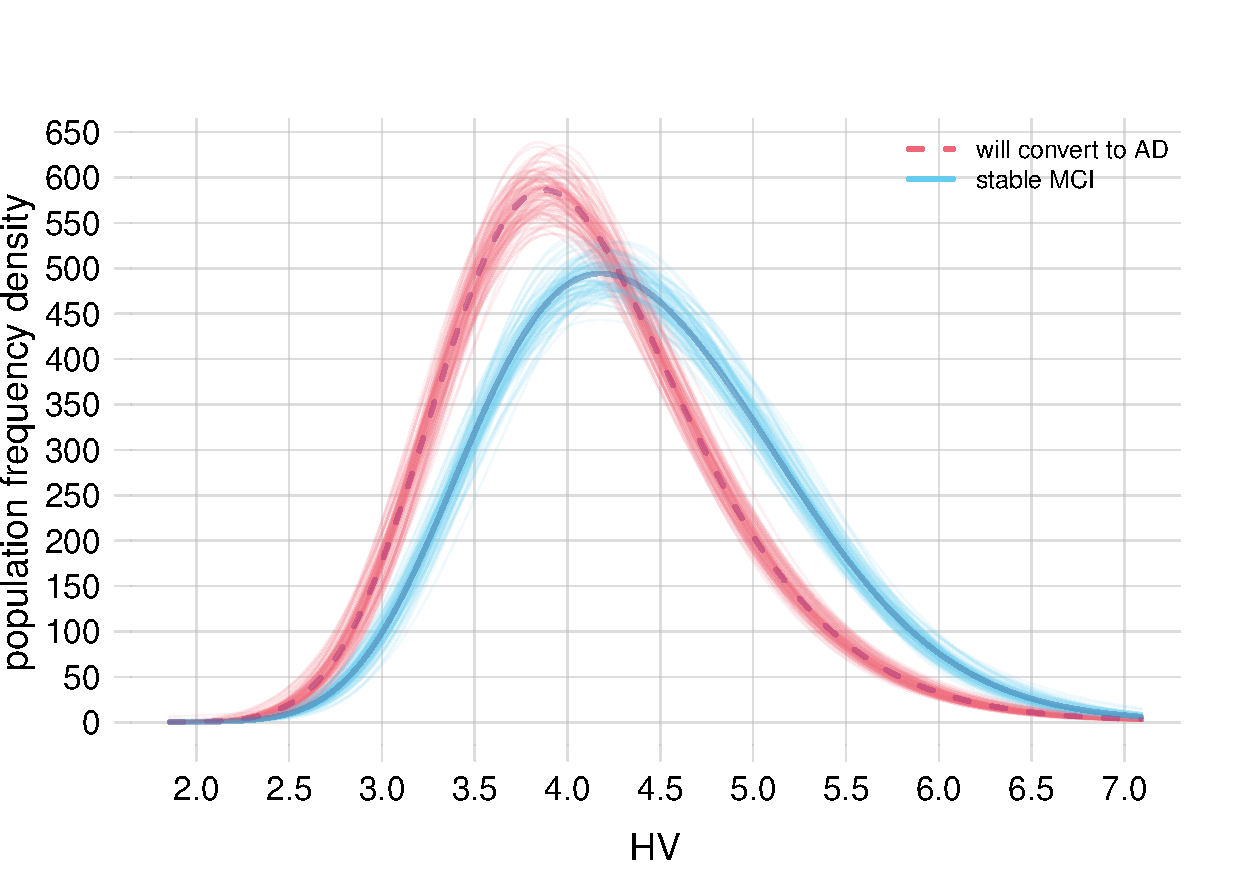
\includegraphics[width=0.45\linewidth]{figures/population_distr_HV.pdf}\hfill%
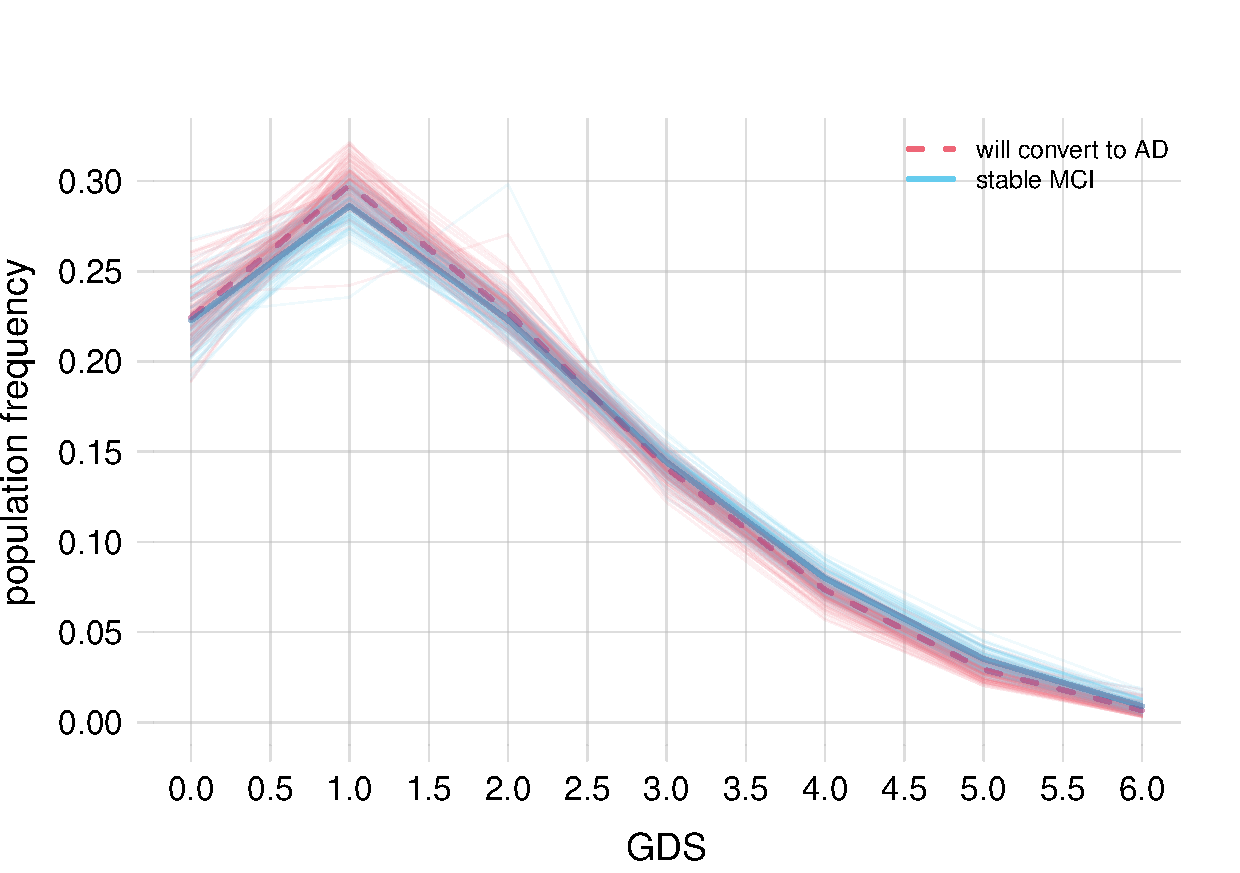
\includegraphics[width=0.45\linewidth]{figures/population_distr_GDS.pdf}%
\\ \caption{}\label{fig:distr}
\end{figure}
The package allows the user to visualize the probabilities above when just one predictand and one predictor variates are involved. If the results of the \texttt{Pr()} function are saved in some object, say \texttt{probs}, then the visualization is done by simply calling \texttt{plot(probs)}.

Figure~\ref{fig:distr} shows two examples from a study \citep{portamanaetal2023b} about conversion from Mild Cognitive Impairment (MCI) to Alzheimer's Disease (AD); they can be used to further illustrate the probability distributions~\eqref{eq:prob_var} and~\eqref{eq:prob_freq}.

In the plot on the left, the predictand variate is Hippocampal Volume ($\HV$); the predictor is the yes/no variate `will convert to AD' ($\cAD$). The thick solid blue line and thick dashed red line are the conditional probability distributions (omitting the sample-data dependence)
\begin{equation*}
  \P( \HV \| \cAD \mo \yn)\ ,\qquad
  \P( \HV \| \cAD \mo \yy) \ .
\end{equation*}
The cloud of thinner blue lines surrounding the first distribution above  represents the probability distribution
\begin{equation*}
  \P\bigl[ \yF(\HV \| \cAD \mo \yn)\bigr]
\end{equation*}
of possible frequency distributions; each thin line is a sample from this distribution.

Looking at this plot, a clinician can immediately see that the frequency distributions of hippocampal volume in the sub-populations of patients that will convert to Alzheimer's, and in those who will not, are different. Such a difference is almost certain even accounting for the uncertainty from the finite sample size. The plot on the right is analogous but for the predictand variate `Geriatric Depression Scale' ($\GDS$) in stead of hippocampal volume. In this case the clinician sees that the frequency distributions for the two sub-populations cannot be distinguished within the finite-sample uncertainty.

It is exactly this kind of differences and uncertainties that clinical researchers often try to clumsily capture through $p$-values. In private communications, several clinical researchers expressed elation at the capacity to visualize the estimates of different sub-population statistics, and even more the uncertainties they carry because of finite sample size.

The quick analysis above is mostly qualitative, but concrete numbers, such as quantiles and credibility intervals, expected values, and so on, can be easily produced. This becomes necessary when many variates are considered jointly and visualization is impossible. In such high-dimensional cases the package allows the user to compute the credibility intervals for any kind of distance between two frequency distributions (e.g. Hellinger or Kantorovich or Shannon-Jansen distance, or relative entropy). The computation of the mutual information between any two sets of variates, illustrated in a vignette\footnote{\url{https://pglpm.github.io/inferno/articles/mutualinfo.html}}, gives moreover a measure of their association that does not depend on assumptions such as linearity or gaussianity.

\begin{figure}[t]
\centering%
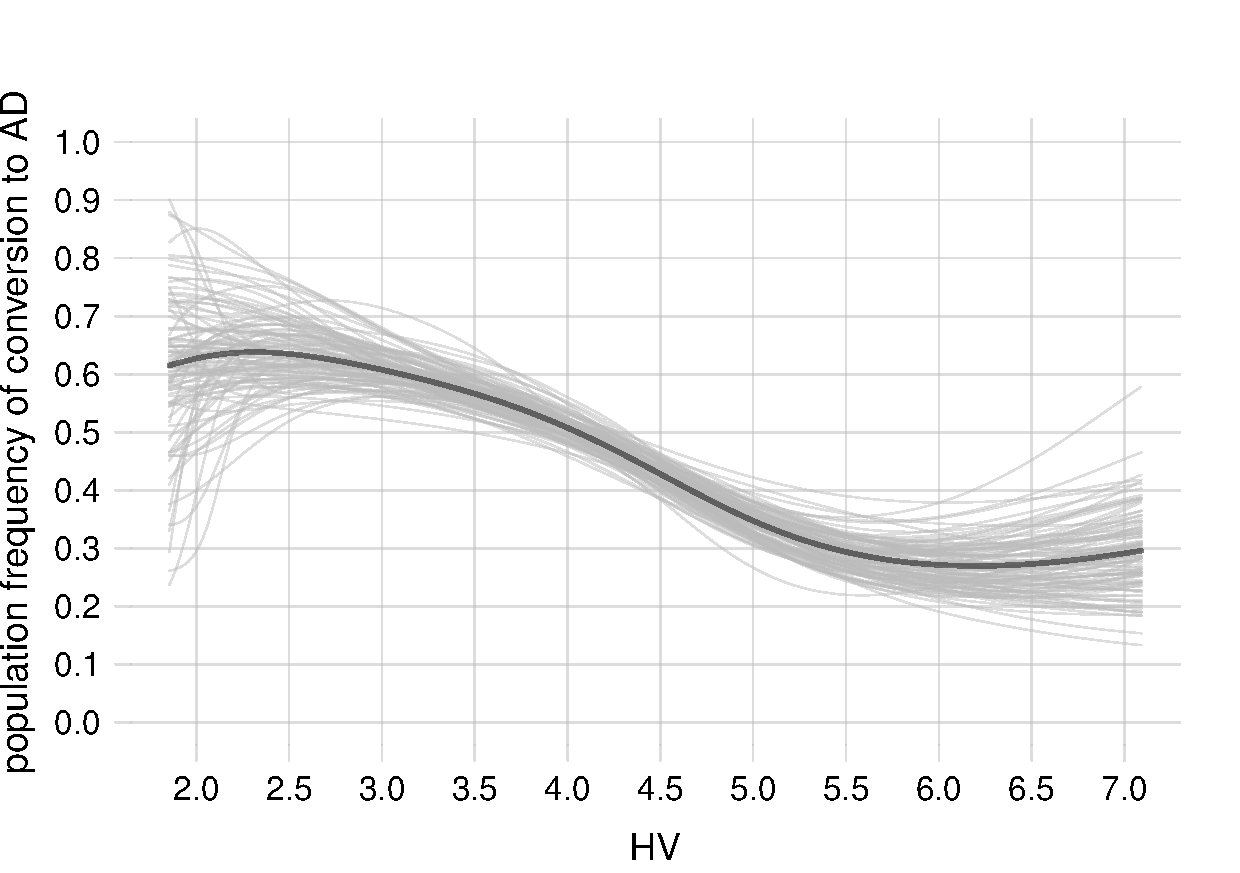
\includegraphics[width=0.45\linewidth]{figures/prob_conversion_HV.pdf}\hfill%
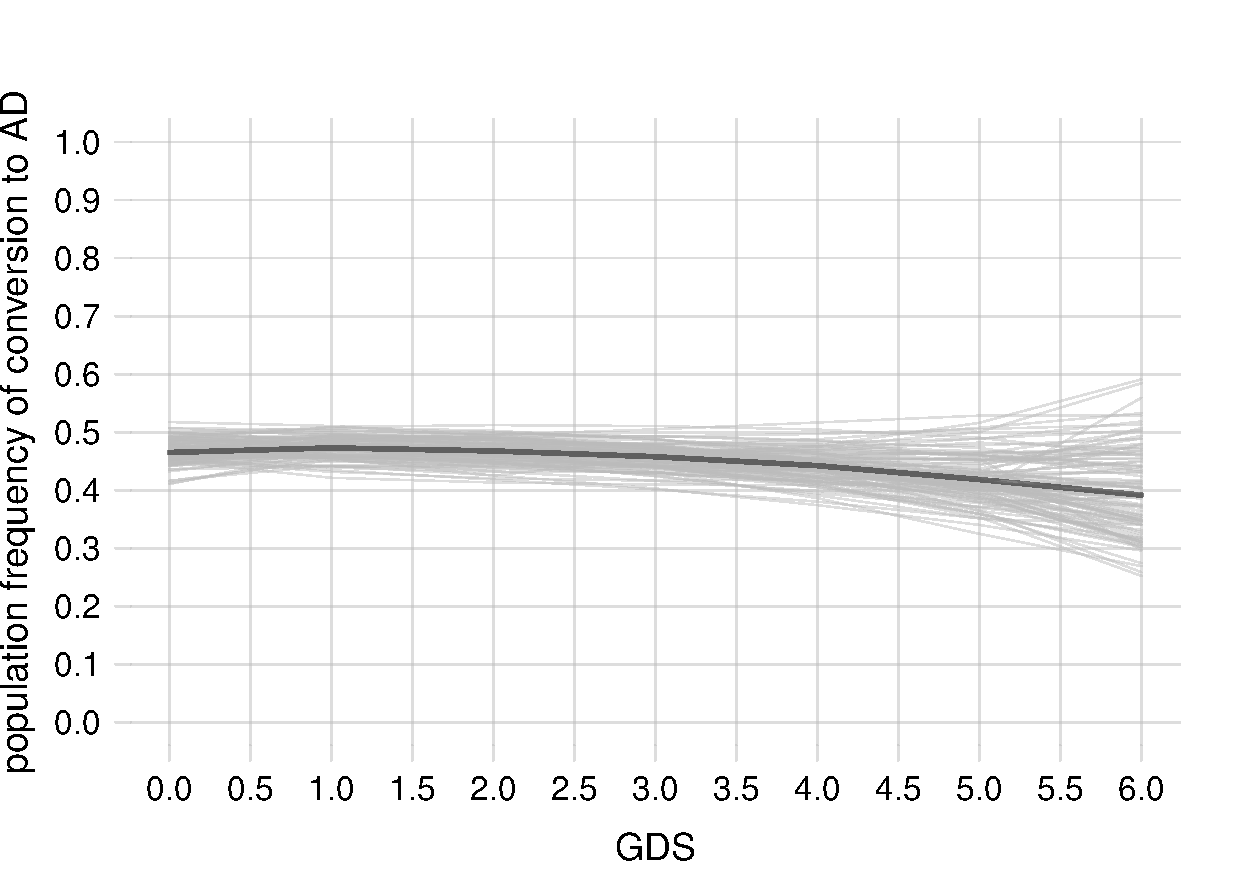
\includegraphics[width=0.45\linewidth]{figures/prob_conversion_GDS.pdf}%
\\ \caption{}\label{fig:distr_inv}
\end{figure}
The ability to swap the ``predictor'' and ``predictand'' roles of any variates is illustrated in the plots of fig.~\ref{fig:distr_inv}, parallel to those of fig.~\ref{fig:distr}. In the left plot, the thicker lines show the probabilities
\begin{equation*}
  \P( \cAD \mo \yy \| \HV)\
%  ,\qquad  \P( \cAD \mo \yy \| \GDS)
\end{equation*}
for various values of the $\HV$ variate, which is now a predictor.
% The clouds of thinner lines are samples of the corresponding probability distributions of the frequency distributions.
We see for example that among individuals having hippocampal volume around $5.0$, between 30\% and 40\% will convert to Alzheimer's. Among those with volume around $2.0$, we can only say that between roughly 45\% and 80\% will convert; in this case the finite-sample size (few samples with this $\HV$ value) leads to a much larger uncertainty of the frequency estimates.

The possibility of swapping predictor and predictand roles makes it also possible to implement, on the fly, corrections for base rates by means of Bayes's theorem \cite[\S\,4]{lindleyetal1981}.%\citep[\S\,3.2]{portamanaetal2023b}.

\medskip

Plots and calculations like the ones above are of course nothing new in Bayesian nonparametrics. The point here is that the user can produce them just by inputting the population sample in the package, waiting for the MCMC computation to finish, and then simply asking about variates of interest and plotting the results. The sequence of commands could be as simple as
\begin{verbatim}
learnt <- learn(data = 'data.csv', metadata = 'metadata.csv')
## Information about MCMC and expected end time...

probs <- Pr(Y = list(A = seq(0, 8, 0.1)), X = list(C = c('yes', 'no')), learnt)

plot(probs)
\end{verbatim}
More extensive use examples are given in the package's main vignette\footnote{\url{https://pglpm.github.io/inferno/articles/inferno_start.html}}. The package has also been used to ``calibrate'' the output of machine-learning algorithms \citep{dyrlandetal2022b}, improving their performance. Readers of the ISBA Bulletin are probably interested in the internals of the package, discussed next.


\subsection*{Internals}
\label{sec:representation}

In nonparametric population inference the prior and posterior probability distributions are over an in-principle infinite-dimensional manifold of frequency distributions. The mathematical representation of this manifold is therefore crucial. The \textbf{inferno} package uses the ingenious representation of a distribution as a mixture of product kernels discussed by Dunson \& Bhattacharya \citeyear{dunsonetal2011}. For example, a generic frequency distribution for variates $A$ and $B$ is written as
\begin{equation}
  \label{eq:mixture_kernel}
  \yF(A, B) = \sum_{i} w_{i}\, K_{A}(A \| \alpha_{i})\, K_{B}(B \| \beta_{i})
\end{equation}
where $w_{i}$ are normalized weights, $K_{A}$ a distribution for variate $A$ depending on parameters $\alpha_{i}$, and similarly for $K_{B}$. The product is easily generalized to any number of variates. In principle the sum should be countably infinite, but as discussed in Ishwaran \& Zarepour \citeyear{ishwaranetal2002c} it is possible to truncate it if an appropriate Dirichlet distribution is used for the weights $w_{i}$. Thus a frequency distribution $\yF$ is effectively represented, non-uniquely, by a very large but finite set of parameters $(w_{i}, \alpha_{i}, \beta_{i})$.

The representation above was somewhat deprecated in recent works which, however, consider inference problems where variates have clear predictor or predictand roles \citep[e.g.][]{wadeetal2014,wadeetal2014b}. As previously discussed, in many research fields there are no such a-priori roles; any variate could assume both. A representation that can easily swap the two roles  without overemphasizing either is therefore most appropriate. The representation~\eqref{eq:mixture_kernel} leads to very simple, symmetric, analytical expressions for the conditional of $A$ given $B$ and vice versa, and for any marginal:
\begin{equation*}
  \begin{gathered}
    \yF(A \| B) = \sum_{i}
    \frac{w_{i}\, K_{A}(A \| \alpha_{i})\, K_{B}(B \| \beta_{i})}{\sum_{j} w_{j}K_{B}(B \| \beta_{j})}
\qquad\qquad    \yF(B \| A) = \sum_{i}
    \frac{w_{i}\, K_{B}(B \| \beta_{i})\, K_{A}(A \| \alpha_{i})}{\sum_{j} w_{j}K_{A}(A \| \alpha_{j})}
    \\
    \yF(A) = \sum_{i}
    w_{i}\, K_{A}(A \| \alpha_{i}) \ .
  \end{gathered}
\end{equation*}
The (hyper)prior over the parameters representing the frequency distribution is a Dirichlet-process mixture. It allows for distributions having multiple, possibly sharp, peaks. For information about the kernels $K$ for different kinds of variates, and about the prior distribution, see the technical manual\footnote{\url{https://github.com/pglpm/inferno/raw/main/development/manual/optimal_predictor_machine.pdf}}.

\smallskip

The MCMC computation is based on Gibbs sampling; several chains are run in parallel. The stopping rule implements variations of the methods discussed in \cite{vehtarietal2021}. Regarding MCMC sampling, the package takes the following stance:

\textbullet\ For this kind of inference problems there is no need for tens of thousands or more independent MCMC samples (effective sample size). The package's default is just 3600. The mean of such samples is the probability~\eqref{eq:prob_var}, and the numerical uncertainty in this mean is thus around $\sqrt{3600} = 60$ times smaller than the ``variability'' of this probability, given by eq.~\eqref{eq:prob_freq}.

\textbullet\ It is acceptable that the sampling has not \emph{fully} converged (emphasis on `fully'). Why? Consider that machine-learning algorithms such as neural networks are effectively Bayesian nonparametric functional regressors, and their training is essentially an \emph{unconverged} Monte Carlo sampling \citep[see e.g.][]{mackay1992b,gal2016,mandtetal2017,huszar2017}. This ``sampling'' stops at a \emph{local} maximum of the posterior, and all samples are discarded. Thanks to this lack of convergence, neural-network training is fast; despite this lack of convergence, inferences can still be impressive. It is this writer's opinion that the same stance can and should at times be adopted in Bayesian nonparametrics: inferences can still be impressive and informative despite lack of full MCMC convergence, and superior to those of many machine-learning algorithms designed for the same task, as we found by using this package. And the uncertainty in the results can moreover be approximately assessed, instead of fully discarded as in neural-network training. So far, in applying \textbf{inferno} to concrete problems, we noticed that the MCMC sampling had converged in the majority of cases. In those in which it had not fully converged, the results were still correct to a good approximation, for example with credibility intervals that erred by less than 2\% from the converged values. This kind of approximate nonparametric results are still vastly superior to precise but opaque $p$-values.

These stances are motivated by the need for user-friendliness. The ultimate goal of the package is to let frequentist practitioners try and appreciate Bayesian methods (the package's main vignette is specially written for them); to let Bayesian-parametric practitioners try nonparametrics; and to show that Bayesian methods can be almost as fast and more powerful than many machine-learning approaches. Once the merits are seen, practitioners can slowly move to more complex Bayesian packages that allow for more control and custom problem-solving.

\textbf{inferno} has been already used and tested in several studies, but we'd like more testing before submitting it to CRAN. Testers and feedback are very welcome!


%{\small\input{preamble.tex}
\newcommand{\citebi}{\cite}
\newcommand{\citein}[1]{\textnormal{\cite{#1}}}
\newcommand*{\subtitleproc}[1]{}
\newcommand*{\chapb}{}
\providecommand{\doi}[1]{}
\renewcommand{\doi}[1]{\href{https://doi.org/#1}{doi:#1}}
\newcommand*{\osfdoi}[1]{Open Science Framework \doi{#1}}
\newcommand*{\arxivdoi}[1]{arXiv \doi{#1}}
\newcommand*{\amp}{\&}
%% Probability macros
\renewcommand*{\P}{\mathrm{P}}%probability
\renewcommand*{\|}[1][]{\nonscript\:#1\vert\nonscript\:\mathopen{}}
\newcommand*{\mo}[1][=]{\mathclose{}\mathord{\nonscript\mkern0.5mu#1\nonscript\mkern0.5mu}\mathopen{}}
\newcommand*{\yF}{F}
\newcommand*{\yf}{f}
\newcommand*{\di}{\mathop{}\!\mathrm{d}}
%%
\newcommand*{\HV}{\mathit{HV}}
\newcommand*{\GDS}{\mathit{GDS}}
\newcommand*{\cAD}{\mathit{cAD}}
\newcommand*{\yy}{\mathrm{Y}}
\newcommand*{\yn}{\mathrm{N}}


\MyFilledBox{SOFTWARE HIGHLIGHT}
\begin{center}
  {\large Luca\enspace Porta Mana} \\
  Western Norway University of Applied Sciences\\
{\tt \href{mailto:pgl@portamana.org}{pgl@portamana.org}}


\Large
\textsc{inferno: INFERence in R with Bayesian NOnparametrics}
\end{center}

\subsection*{Population inference and Bayesian nonparametrics}
\label{sec:popinference}

A very important kind of inference in research fields such as medicine is \emph{population inference}, also called ``density inference'' or ``density regression''. Its general goal is to infer the frequency distribution of some variates in a population. This is different, for instance, from \emph{functional regression}, where the goal is to infer the functional relationship -- assumed to exist -- between a set of predictor variates and a target or ``predictand'' variate. In population inference the existence of a functional relation cannot be assumed. In fact there may not even be a clear distinction between predictor and predictand variates. A typical goal is the inference of frequency distributions within particular sub-populations or sub-groups; thus all sorts of conditional probabilities are required. A clinician may be interested in the statistics and probability of a medical condition given a symptom, but also in that of a symptom given a medical condition; and maybe only within subjects of a given sex or age. De~Finetti's theorem \citep[see e.g.][\S\S\,4.2, 4.3, 4.6]{bernardoetal1994_r2000} lies at the heart of population-inference methods; a particularly brilliant discussion is given by Lindley \& Novick \citeyearpar{lindleyetal1981}.

Sadly many researchers still approach population-inference problems by means of $p$-values or other frequentist practices, which only give limited, coarse, and not seldom misleading results about a population's frequency distribution. Some researchers adopt Bayesian methods but limit themselves to \emph{parametric} ones, which make very restrictive and possibly unrealistic assumptions about the population's distribution; as opposed to \emph{nonparametric} ones, which do not.

Until a couple decades ago the use of parametric methods, and maybe even of frequentist practices, had pragmatic reasons. Better methods were computationally too costly or unfeasible. Population-inference problems were low-dimensional; one could \emph{visually} check whether the assumptions were appropriate and the results reasonable. But today these reasons cannot earnestly be given \citep{walker2010}. Bayesian nonparametric methods have become computationally feasible for many kinds of inference. Many inference problems today involve from tens to thousands of variates; it is impossible to visually check in such high-dimensional spaces whether frequentist practices or parametric assumptions are acceptable, or by how much they err. Results may be affected by large parametric-modelling errors \citep{draper1995}.

But there is still one reason today for why Bayesian nonparametric methods are avoided: \emph{lack of user-friendly software}. Many clinical researchers might like to try a Bayesian nonparametric analysis, but cannot: they would need to study Markov-chain Monte Carlo (MCMC) techniques, programming languages to implement the latter, and a read about plethora of debated practices to ``assess convergence''. Most clinicians do not have time to learn all this even if they wanted to. Also, available packages for Bayesian nonparametrics are not quite suited to population inference. Some of them focus on functional regression, which as discussed above is not an appropriate assumption. Some make a priori distinctions between predictor and predictand variates, limiting the range of useful inferences. Most still require MCMC programming expertise.

The R-package \textbf{inferno}\footnote{\url{https://pglpm.github.io/inferno/}} was built to try to remedy the lack of user-friendly software of this kind.

\subsection*{Use and features}
\label{sec:features}

Using the package is simple. The user first provides a data sample $S$ of variates from a population, for instance age, sex, symptom, disease, and kind of treatment of a number of patients that satisfy specific criteria. The package can work with any combination of continuous, discrete ordinal, nominal, and binary variates. Continuous variates can be defined in bounded intervals, and can also have boundary values with finite probability mass, as it may happen with censoring. The package cannot handle periodic variates yet, or variates with complex topology, such as images. The data sample and the variate characteristics (type, domain, possible censoring) are provided by the user as two CSV files to an R function called \texttt{learn()}.

The package then runs a MCMC computation by means of the \textbf{Nimble} package\footnote{\url{https://r-nimble.org/}}, using parallel CPUs if available, to find the probability distribution over all possible joint frequency distributions of the variates. The result is saved in an R object called \texttt{learnt}. The crucial point here is that this computation is automatic and does not require any further control from the user, who is simply informed at regular intervals about the expected end time of the computation. (Optional arguments still allow users expert in MCMC to control many parameters such as number of chains, target effective sample size, thinning and burn-in, and even some hyperprior parameters.)

Once the computation has finished, the user can inquire multiple times about any of the following:
\vspace{-\topsep}
\setlength{\leftmargini}{17.62pt}
\begin{itemize}
  \itemsep0.5ex
\item For a new unit of the population, say a new patient, the conditional probability (density) for the values of \emph{any} set of variates $A \mo a, B \mo b, \dotso$ given \emph{any} other set $C \mo c, D \mo d, \dotso$:
  \begin{equation}\label{eq:prob_var}
    \P(A \mo a, B \mo b, \dotso \|C \mo c, D \mo d, \dotso , S)
  \end{equation}
  Such a probability could for instance be used in medical decision making \citep{soxetal1988_r2024,huninketal2001_r2014}. The conditional can be empty; tail probabilities (e.g.\ $A \ge a$, $C \le c$) can also be requested.

\item The probability distribution for the conditional \emph{frequencies}, in the whole unsampled population, of the values of any set of variates given any other set (possibly empty). If we denote the frequency distribution by $\yF$ and a specific value by $\yf$, this probability can be written
  \begin{equation}\label{eq:prob_freq}
    \P\bigl[ \yF(A \mo a, \dotso \|C \mo c, \dotso) = \yf \|[\big] S\bigr]
    \,\di\yf \ .
  \end{equation}
This probability distribution is represented by the MCMC samples $\yf_{i}$ drawn from it by \texttt{learn()}.

\item The mutual information \citep[Ch.~8]{mackay1995_r2005} between any two sets of quantities.
\end{itemize}
\vspace{-\topsep}

Probabilities~\eqref{eq:prob_var} and~\eqref{eq:prob_freq} are connected by a variant of de~Finetti's theorem:
\begin{equation}
  \label{eq:definetti1}
  \P(A \mo a, \dotso \|C \mo c, \dotso , S)  =
  \int \yf \,
  \P\bigl[ \yF(A \mo a, \dotso \|C \mo c, \dotso) = \yf \|[\big] S\bigr]
  \,\di\yf \ .
\end{equation}

In a manner of speaking, the probability distribution~\eqref{eq:prob_freq} expresses how much the probability value~\eqref{eq:prob_var} could change, if it were updated by sampling the whole population. It expresses the uncertainty in the statistical results owing to finite sample size.

The package function \texttt{Pr(Y, X, learnt)} does the first two kinds of calculations. The user provides a list \texttt{Y} of predictand variates and values of interest; an optional, analogous list \texttt{X} of predictors; and the \texttt{learnt} object produced by \texttt{learn()}. The calculation of mutual information is done by the package function \texttt{mutualinfo(Y1names, Y2names, X)}, where the first two arguments are the variate sets of interest, and the optional third argument is a set of variate values to conditionalize upon.

\medskip

\begin{figure}[t]
\centering%
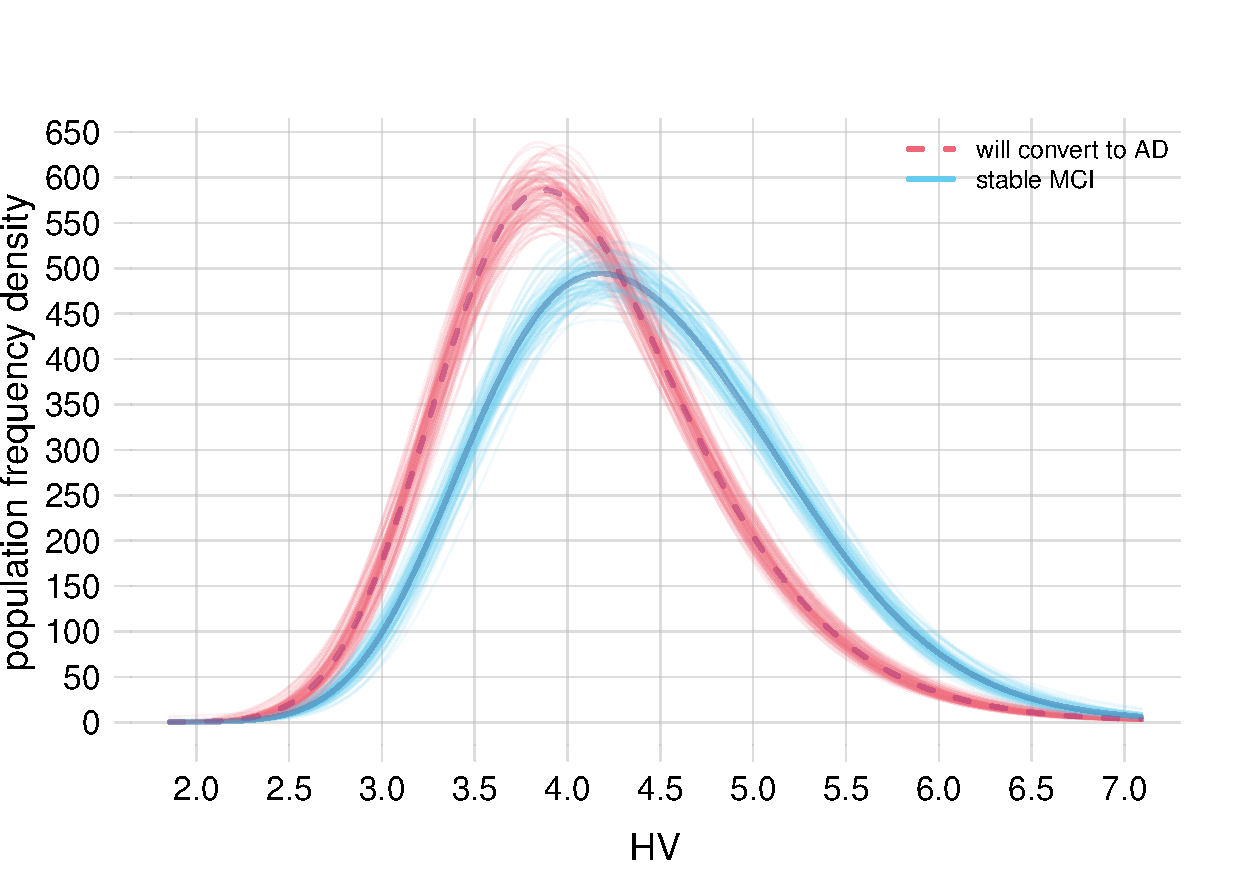
\includegraphics[width=0.45\linewidth]{figures/population_distr_HV.pdf}\hfill%
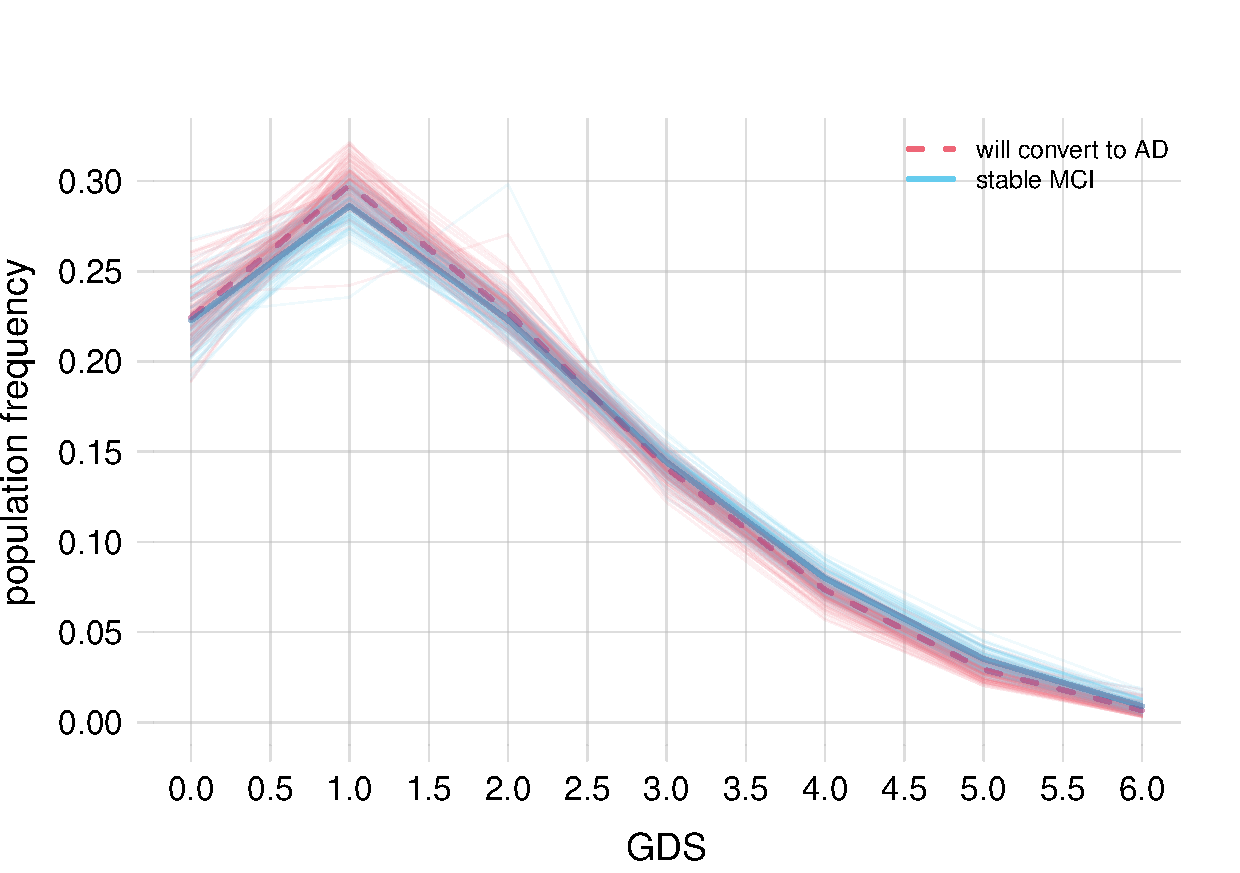
\includegraphics[width=0.45\linewidth]{figures/population_distr_GDS.pdf}%
\\ \caption{}\label{fig:distr}
\end{figure}
The package allows the user to visualize the probabilities above when just one predictand and one predictor variates are involved. If the results of the \texttt{Pr()} function are saved in some object, say \texttt{probs}, then the visualization is done by simply calling \texttt{plot(probs)}.

Figure~\ref{fig:distr} shows two examples from a study \citep{portamanaetal2023b} about conversion from Mild Cognitive Impairment (MCI) to Alzheimer's Disease (AD); they can be used to further illustrate the probability distributions~\eqref{eq:prob_var} and~\eqref{eq:prob_freq}.

In the plot on the left, the predictand variate is Hippocampal Volume ($\HV$); the predictor is the yes/no variate `will convert to AD' ($\cAD$). The thick solid blue line and thick dashed red line are the conditional probability distributions (omitting the sample-data dependence)
\begin{equation*}
  \P( \HV \| \cAD \mo \yn)\ ,\qquad
  \P( \HV \| \cAD \mo \yy) \ .
\end{equation*}
The cloud of thinner blue lines surrounding the first distribution above  represents the probability distribution
\begin{equation*}
  \P\bigl[ \yF(\HV \| \cAD \mo \yn)\bigr]
\end{equation*}
of possible frequency distributions; each thin line is a sample from this distribution.

Looking at this plot, a clinician can immediately see that the frequency distributions of hippocampal volume in the sub-populations of patients that will convert to Alzheimer's, and in those who will not, are different. Such a difference is almost certain even accounting for the uncertainty from the finite sample size. The plot on the right is analogous but for the predictand variate `Geriatric Depression Scale' ($\GDS$) in stead of hippocampal volume. In this case the clinician sees that the frequency distributions for the two sub-populations cannot be distinguished within the finite-sample uncertainty.

It is exactly this kind of differences and uncertainties that clinical researchers often try to clumsily capture through $p$-values. In private communications, several clinical researchers expressed elation at the capacity to visualize the estimates of different sub-population statistics, and even more the uncertainties they carry because of finite sample size.

The quick analysis above is mostly qualitative, but concrete numbers, such as quantiles and credibility intervals, expected values, and so on, can be easily produced. This becomes necessary when many variates are considered jointly and visualization is impossible. In such high-dimensional cases the package allows the user to compute the credibility intervals for any kind of distance between two frequency distributions (e.g. Hellinger or Kantorovich or Shannon-Jansen distance, or relative entropy). The computation of the mutual information between any two sets of variates, illustrated in a vignette\footnote{\url{https://pglpm.github.io/inferno/articles/mutualinfo.html}}, gives moreover a measure of their association that does not depend on assumptions such as linearity or gaussianity.

\begin{figure}[t]
\centering%
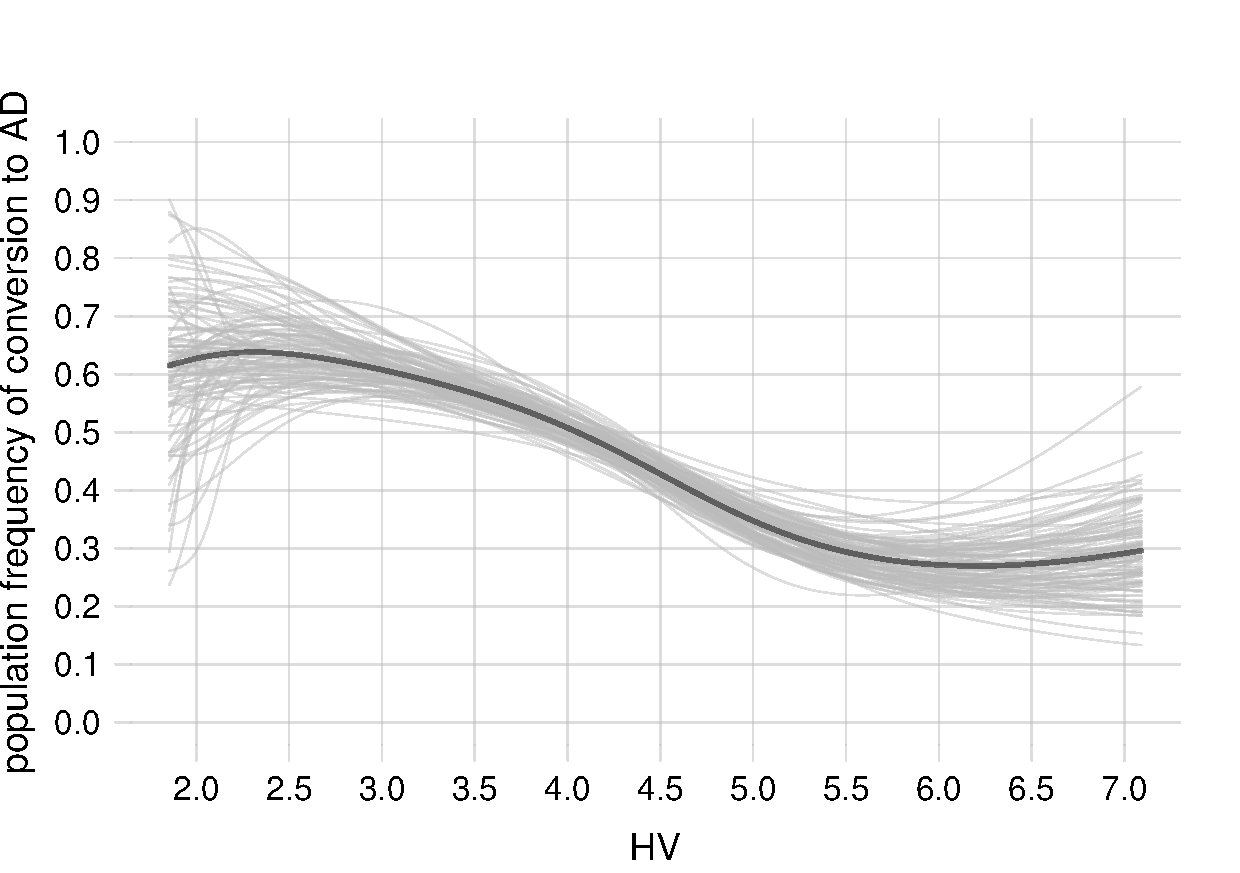
\includegraphics[width=0.45\linewidth]{figures/prob_conversion_HV.pdf}\hfill%
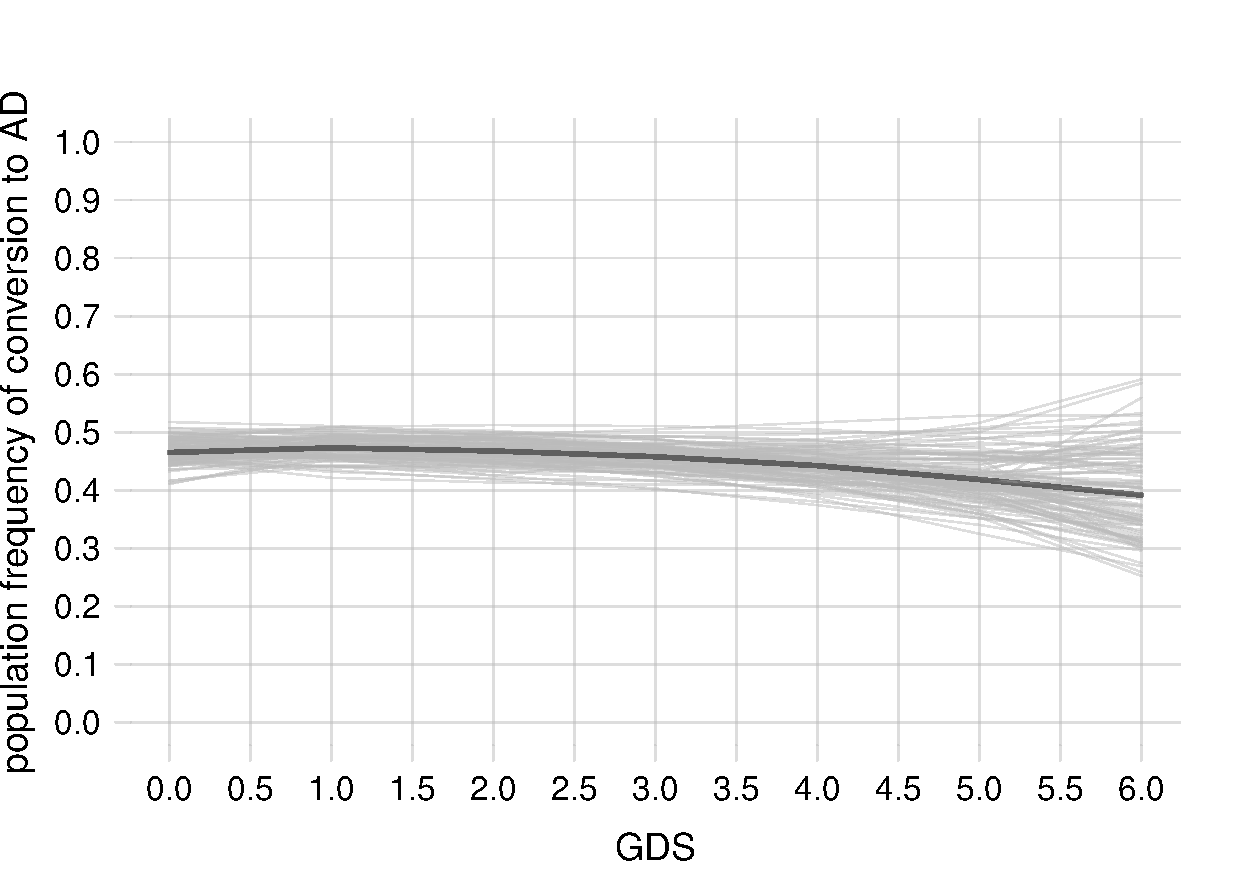
\includegraphics[width=0.45\linewidth]{figures/prob_conversion_GDS.pdf}%
\\ \caption{}\label{fig:distr_inv}
\end{figure}
The ability to swap the ``predictor'' and ``predictand'' roles of any variates is illustrated in the plots of fig.~\ref{fig:distr_inv}, parallel to those of fig.~\ref{fig:distr}. In the left plot, the thicker lines show the probabilities
\begin{equation*}
  \P( \cAD \mo \yy \| \HV)\
%  ,\qquad  \P( \cAD \mo \yy \| \GDS)
\end{equation*}
for various values of the $\HV$ variate, which is now a predictor.
% The clouds of thinner lines are samples of the corresponding probability distributions of the frequency distributions.
We see for example that among individuals having hippocampal volume around $5.0$, between 30\% and 40\% will convert to Alzheimer's. Among those with volume around $2.0$, we can only say that between roughly 45\% and 80\% will convert; in this case the finite-sample size (few samples with this $\HV$ value) leads to a much larger uncertainty of the frequency estimates.

The possibility of swapping predictor and predictand roles makes it also possible to implement, on the fly, corrections for base rates by means of Bayes's theorem \cite[\S\,4]{lindleyetal1981}.%\citep[\S\,3.2]{portamanaetal2023b}.

\medskip

Plots and calculations like the ones above are of course nothing new in Bayesian nonparametrics. The point here is that the user can produce them just by inputting the population sample in the package, waiting for the MCMC computation to finish, and then simply asking about variates of interest and plotting the results. The sequence of commands could be as simple as
\begin{verbatim}
learnt <- learn(data = 'data.csv', metadata = 'metadata.csv')
## Information about MCMC and expected end time...

probs <- Pr(Y = list(A = seq(0, 8, 0.1)), X = list(C = c('yes', 'no')), learnt)

plot(probs)
\end{verbatim}
More extensive use examples are given in the package's main vignette\footnote{\url{https://pglpm.github.io/inferno/articles/inferno_start.html}}. The package has also been used to ``calibrate'' the output of machine-learning algorithms \citep{dyrlandetal2022b}, improving their performance. Readers of the ISBA Bulletin are probably interested in the internals of the package, discussed next.


\subsection*{Internals}
\label{sec:representation}

In nonparametric population inference the prior and posterior probability distributions are over an in-principle infinite-dimensional manifold of frequency distributions. The mathematical representation of this manifold is therefore crucial. The \textbf{inferno} package uses the ingenious representation of a distribution as a mixture of product kernels discussed by Dunson \& Bhattacharya \citeyear{dunsonetal2011}. For example, a generic frequency distribution for variates $A$ and $B$ is written as
\begin{equation}
  \label{eq:mixture_kernel}
  \yF(A, B) = \sum_{i} w_{i}\, K_{A}(A \| \alpha_{i})\, K_{B}(B \| \beta_{i})
\end{equation}
where $w_{i}$ are normalized weights, $K_{A}$ a distribution for variate $A$ depending on parameters $\alpha_{i}$, and similarly for $K_{B}$. The product is easily generalized to any number of variates. In principle the sum should be countably infinite, but as discussed in Ishwaran \& Zarepour \citeyear{ishwaranetal2002c} it is possible to truncate it if an appropriate Dirichlet distribution is used for the weights $w_{i}$. Thus a frequency distribution $\yF$ is effectively represented, non-uniquely, by a very large but finite set of parameters $(w_{i}, \alpha_{i}, \beta_{i})$.

The representation above was somewhat deprecated in recent works which, however, consider inference problems where variates have clear predictor or predictand roles \citep[e.g.][]{wadeetal2014,wadeetal2014b}. As previously discussed, in many research fields there are no such a-priori roles; any variate could assume both. A representation that can easily swap the two roles  without overemphasizing either is therefore most appropriate. The representation~\eqref{eq:mixture_kernel} leads to very simple, symmetric, analytical expressions for the conditional of $A$ given $B$ and vice versa, and for any marginal:
\begin{equation*}
  \begin{gathered}
    \yF(A \| B) = \sum_{i}
    \frac{w_{i}\, K_{A}(A \| \alpha_{i})\, K_{B}(B \| \beta_{i})}{\sum_{j} w_{j}K_{B}(B \| \beta_{j})}
\qquad\qquad    \yF(B \| A) = \sum_{i}
    \frac{w_{i}\, K_{B}(B \| \beta_{i})\, K_{A}(A \| \alpha_{i})}{\sum_{j} w_{j}K_{A}(A \| \alpha_{j})}
    \\
    \yF(A) = \sum_{i}
    w_{i}\, K_{A}(A \| \alpha_{i}) \ .
  \end{gathered}
\end{equation*}
The (hyper)prior over the parameters representing the frequency distribution is a Dirichlet-process mixture. It allows for distributions having multiple, possibly sharp, peaks. For information about the kernels $K$ for different kinds of variates, and about the prior distribution, see the technical manual\footnote{\url{https://github.com/pglpm/inferno/raw/main/development/manual/optimal_predictor_machine.pdf}}.

\smallskip

The MCMC computation is based on Gibbs sampling; several chains are run in parallel. The stopping rule implements variations of the methods discussed in \cite{vehtarietal2021}. Regarding MCMC sampling, the package takes the following stance:

\textbullet\ For this kind of inference problems there is no need for tens of thousands or more independent MCMC samples (effective sample size). The package's default is just 3600. The mean of such samples is the probability~\eqref{eq:prob_var}, and the numerical uncertainty in this mean is thus around $\sqrt{3600} = 60$ times smaller than the ``variability'' of this probability, given by eq.~\eqref{eq:prob_freq}.

\textbullet\ It is acceptable that the sampling has not \emph{fully} converged (emphasis on `fully'). Why? Consider that machine-learning algorithms such as neural networks are effectively Bayesian nonparametric functional regressors, and their training is essentially an \emph{unconverged} Monte Carlo sampling \citep[see e.g.][]{mackay1992b,gal2016,mandtetal2017,huszar2017}. This ``sampling'' stops at a \emph{local} maximum of the posterior, and all samples are discarded. Thanks to this lack of convergence, neural-network training is fast; despite this lack of convergence, inferences can still be impressive. It is this writer's opinion that the same stance can and should at times be adopted in Bayesian nonparametrics: inferences can still be impressive and informative despite lack of full MCMC convergence, and superior to those of many machine-learning algorithms designed for the same task, as we found by using this package. And the uncertainty in the results can moreover be approximately assessed, instead of fully discarded as in neural-network training. So far, in applying \textbf{inferno} to concrete problems, we noticed that the MCMC sampling had converged in the majority of cases. In those in which it had not fully converged, the results were still correct to a good approximation, for example with credibility intervals that erred by less than 2\% from the converged values. This kind of approximate nonparametric results are still vastly superior to precise but opaque $p$-values.

These stances are motivated by the need for user-friendliness. The ultimate goal of the package is to let frequentist practitioners try and appreciate Bayesian methods (the package's main vignette is specially written for them); to let Bayesian-parametric practitioners try nonparametrics; and to show that Bayesian methods can be almost as fast and more powerful than many machine-learning approaches. Once the merits are seen, practitioners can slowly move to more complex Bayesian packages that allow for more control and custom problem-solving.

\textbf{inferno} has been already used and tested in several studies, but we'd like more testing before submitting it to CRAN. Testers and feedback are very welcome!


%{\small\input{software.bbl}}

\bibliographystyle{abbrvnat}
{\small
\bibliography{software.bib}
}
\end{document}

}

\bibliographystyle{abbrvnat}
{\small
\bibliography{software.bib}
}
\end{document}

}

\bibliographystyle{abbrvnat}
{\small
\bibliography{software.bib}
}
\end{document}

}

\bibliographystyle{abbrvnat}
{\small
\bibliography{software.bib}
}
\end{document}

